\documentclass[11pt]{article}
\usepackage[utf8]{inputenc}
\usepackage[T1]{fontenc} 
\usepackage[french]{babel}
\usepackage{graphicx}
\usepackage{subcaption}
\usepackage[table]{xcolor}
\usepackage{longtable}
\usepackage{geometry}
\usepackage{hyperref}
\usepackage{appendix}
\usepackage{pdfpages}

\geometry{hmargin=2.5cm,vmargin=3cm}
\setlength{\parskip}{0.15cm}

\title{\textbf{Rapport de Stage :\\ Gestion de données de capteurs physiologiques pour un jeu pervasif capable de s'adapter dynamiquement aux états émotionnels du joueur}}
\author{Laureline MARTIN}
\date{Mercredi 7 Octobre 2020}

\begin{document}
\maketitle
\begin{center}
	\Large{Master 2 Data Management in a Digital World - DataScale\\ 
		Université Versailles Saint-Quentin - Paris Saclay\bigskip\\
		Laboratoire CEDRIC\\ 
		Conservatoire National des Arts et Métiers de Paris}
\end{center}
\vfill
\begin{center}
	
\includegraphics[scale=0.25]{../include/uvsq.png}
	
\includegraphics[scale=0.56]{../include/logo-cedric.PNG}\\
\end{center}
\vfill
\begin{center}
	\textbf{Responsables du Master :}
\end{center}
\begin{tabular}{p{4cm}p{4.5cm}p{7.5cm}}
	\hspace*{-1cm}
	Mme Zoubida KEDAD & Maître de conférences & Laboratoire DAVID (équipe \textit{ADAM})\\
	\hspace*{-1cm}
	M. Philippe PUCHERAL & Professeur & Laboratoire DAVID et INRIA (équipe \textit{PETRUS})
\end{tabular}\par
\begin{center}
	\textbf{Encadrants :}
\end{center}
\begin{tabular}{lp{4.5cm}p{7.5cm}}
	\hspace*{-1cm}
	Mme Viviane GAL & Docteur - Ingénieur & Equipe \textit{Interactivité pour lire et jouer - ILJ}\\
	\hspace*{-1cm}
	M. Eric GRESSIER-SOUDAN & Professeur des Universités & Equipe \textit{Réseaux et Objets Connectés - ROC}\\
	\hspace*{-1cm}
	Mme Elena KORNYSHOVA & Maître de conférences & Equipe \textit{Igénieurie des systèmes d'information et de décision - ISID}
\end{tabular}

\newpage
\begin{center}
	\textbf{Résumé :}
\end{center}
\hspace*{0.4cm}
Durant cinq mois et demi, j'ai travaillé au sein du  laboratoire de recherche CEDRIC au Conservatoire National des Arts et Métiers de Paris.\par
Ce stage s'est inscrit dans le projet exploratoire "Conception et développement des jeux pervasifs adaptables avec la prise en compte des états émotionnels des joueurs" du laboratoire. 
L'objectif global de ce projet est de proposer un jeu pervasif où le joueur et ses émotions sont au cœur même du jeu. 
Pour cela, des capteurs physiologiques sont utilisés pour détecter et reconnaître les états émotionnels du joueur. Ainsi que, des capteurs placés dans l'environnement pour connaître le contexte global. 
Ces capteurs génèrent beaucoup de données qu'il faut traiter en temps-réel pour une adaptation dynamique du jeu.
Dans ce rapport, nous proposons une solution pouvant ingérer les données provenant de capteurs physiologiques en temps-réel.
Ensuite, cette solution envoie ces données à des algorithmes déjà existant qui permettent de déduire des états émotionnels.
Un état de l'art ainsi qu'une première version d'une ontologie afin de répondre à cet objectif ont été proposées et se trouvent dans ce rapport.
\vfill
\begin{center}
	\textbf{Abstract :}
\end{center}
\hspace*{0.4cm}
I worked for the CEDRIC research laboratory based in the Conservatoire National des Arts et Métiers in Paris for five and a half months.\par
This internship was registered in the laboratory's exploratory project «Design and development of adaptable pervasive games, while considering the players' emotional states".
The project’s purpose is to develop a pervasive game, where the player and his emotions are the heart of the game.
To reach this goal, physiological sensors are used to detect and recognize the player's emotional states.  Also, other sensors are placed in the environment to understand the global context.
These sensors generate a lot of data that must be processed in real-time for the game to be adapted dynamically. 
This report suggests a solution able to ingest in real-time data coming from physiological sensors.
Then, this solution sends data to existing algorithms capable of detecting and recognizing emotional states.
A state of the art as well as the first version of an ontology to answer this objective are laid out in this document. 


\newpage
\begin{center}
	\textbf{Avant-propos}
\end{center}
\hspace*{0.4cm}
Dans le cadre de la validation du Master 2 Data Managment in a Digital World - Datascale, proposé par l'Université de Versailles Saint-Quentin / Paris Saclay, j'ai effectué un stage de cinq mois et demi du 16 Mars 2020 au 30 Septembre 2020.
Le contexte particulier lié à la crise sanitaire m'a amené à travailler, pour la majorité de mon stage, en télétravail (du 16 Mars au 10 Septembre).\par
Pour communiquer pendant cette période de travail à distance, nous utilisions les mails et nous avons organisé des réunions via Teams tous les 7 à 15 jours.
Ces réunions duraient entre une demie heure et une heure.
Ces sessions vidéos étaient l'occasion de faire le point sur l'avancement de mon travail et sur les tâches des jours à venir.
Cependant, la barrière de l'écran a créé un réel manque de spontanéité lors de nos échanges.
Pour ma part, je pense que les visio-conférences n'ont pas suffit pour échanger tout au long de cette période de télétravail. 
Peut-être qu'une autre forme de communication, comme une messagerie instantanée, ajoutée à celle des réunions sur Teams, aurait pu réduire se manque de spontanéité.\par
A l'issue de ce stage, je pense que les réunions en présentiel restent la meilleure manière de communiquer et de partager autour d'un projet.

\newpage
\renewcommand{\contentsname}{Table des matières}\tableofcontents

\newpage
\section{Introduction}
	Depuis plusieurs années, les jeux pervasifs se multiplient sur le marché, proposant aux joueurs des contenus très immersifs.
	Le jeu pervasif (aussi appelé jeu omniprésent) est un genre de jeu qui mêle le monde physique et le monde numérique et rend floue cette frontière.
	Dans le jeu pervasif, le contexte est essentiel.
	Comme le montre \cite{astic_2013}, quatre facteurs sont mis en jeu : l'espace, le temps, la technologie et les rapports sociaux.
	L'espace du jeu pervasif est à la fois ancré dans le réel et dans le virtuel.
	Il convient alors que des ponts existent entre ces deux espaces.
	Ces ponts peuvent se faire via des objets, des points géographiques, des personnes, etc.
	Le temps est calqué sur le temps réel mais il peut être utilisé de différentes manières dans le jeu.
	Par exemple, l'heure et/ou le jour peuvent influencer le comportement que doit adopter le joueur.
	La technologie est également importante.
	Elle doit rester accessible au joueur, tant sur le plan pratique que sur le plan financier.
	La géolocalisation, les réseaux sans fil (réseaux mobiles, WIFI, bluetooth,...), etc. sont des technologies utilisées pour ce type de jeu.
	Dans les jeux pervasifs, les joueurs, les spectateurs et les non-joueurs sont mélangés dans le même espace.
	Les joueurs n'ont pas de caractéristiques particulières pour se reconnaître.
	Le jeu pervasif a un impact social et culturel important.
	Il favorise les rencontres dans l'espace physique.
	Il permet de découvrir de nouveaux endroits, de nouvelles choses et de s'enrichir culturellement.
	Cependant, le jeu omniprésent ne met pas réellement le joueur au centre de jeu.\par
	Le projet "Conception et développement des jeux pervasifs adaptables avec la prise en compte des états émotionnels des joueurs" vise à mettre le joueur et ses émotions au centre du jeu.
	Ce seront les émotions du joueur qui influenceront le jeu et ses événements.
	Pour pouvoir détecter et reconnaître les états émotionnels du joueur afin que le jeu s'y adapte et propose l'événement le plus adéquat, de multiples capteurs physiologiques peuvent être utilisés.
	Ces capteurs génèrent beaucoup de données qui doivent être stockées et traitées.
	Ces données permettront à des algorithmes de reconnaître les états émotionnels des joueurs tout au long du jeu.\par
	Le but de ce travail a été de dresser le contour d'un jeu pervasif adaptable aux états émotionnels du joueur et d'en affiner la conceptualisation.
	Dans ce rapport, nous nous sommes intéressés, d'une part, à l'adaptation de jeux selon le contexte émotionnel et d'autre part, à la gestion de données générées par des capteurs physiologiques.\par
	Tout d'abord, nous décrirons dans la Section \ref{sec:projet}, notre projet, ses objectifs et la problématique scientifique que nous traiterons dans notre travail et à travers ce rapport.
	Nous présenterons, dans la Section \ref{sec:etatart}, l'état de l'art que nous avons rédigé et plus particulièrement le cadre de comparaison que nous avons mis au point pour l'adaptation dynamique de jeux à leurs joueurs. 
	Nous aborderons dans la Section \ref{sec:escape} la notion d'expérience utilisateur et l'expérience que nous avons menée lors d'un escape game.
	Dans la Section \ref{sec:modelisation}, nous présenterons une ontologie, en cours de construction, d'un jeu pervasif prenant en compte l'état émotionnel du joueur et le bilan que nous tirons de cet exercice.
	Enfin, nous expliquerons dans la Section \ref{sec:prototypage} une solution que nous avons conçue pour la gestion de données en temps-réel provenant de capteurs physiologiques.




\section{Cadre du projet}\label{sec:projet}
	Le projet exploratoire intitulé "Conception et développement des jeux pervasifs adaptables avec la prise en compte des états émotionnels des joueurs" a éé initié par Mme Viviane GAL (équipe ILJ, voir Annexe \ref{ann:cedric}), M. Eric GRESSIER-SOUDAN (équipe ROC) et Mme Elena KORNYSHOVA (équipe ISID).
	Ce projet vise à élaborer un jeu pervasif capable de s'adapter dynamiquement selon le contexte du joueur et de son environnement au cours du jeu.\par
	Dans cette section, nous présentons l'objectif global de ce projet.
	Puis, nous présentons la problématique scientifique à laquelle nous apporterons notre contribution.
	Nous donnons aussi des définitions essentielles pour les notions clés et nous abordons les sujets connexes que nous verrons tout au long de ce rapport.
	\subsection{Motivations et objectif du projet}\label{sec:objectif}
		Avec le jeu pervasif, il est possible de créer une grande immersion et une plus grande implication (i.e. engagement) du joueur pour le jeu en comparaison d'autres types de jeux tels que les jeux vidéo ou les jeux de société.
		L'idée principale de notre projet est de concevoir un jeu omniprésent capable de détecter et de reconnaître dynamiquement l'état émotionnel courant de joueur.
		Le jeu devra aussi être capable de s'adapter à cet état en temps-réel en proposant un événement spécifique.
		La Figure \ref{fig:motivation} schématise l'objectif de notre projet.
		\begin{figure}{h}
			\centering
			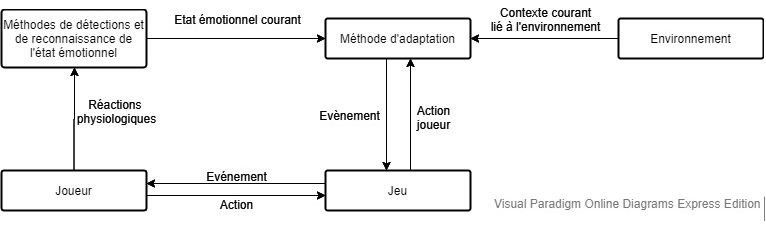
\includegraphics[scale=0.75]{../include/motivation.jpg}
			\caption{Objectif global du projet}
			\label{fig:motivation}
		\end{figure}
		Un joueur qui jouera à notre jeu aura une ou des réaction(s) physiologique(s) qui traduiront un état émotionnel détecté et reconnu par nos algorithmes \cite{gal_2019,gal_et_al._2020}.
		Cet état émotionnel courant sera indiqué à nos algorithmes d'adaptations qui recevront aussi des indications sur l'état courant de l'environnement et sur les actions que fait le joueur dans le jeu.
		Les algorithmes d'adaptation indiqueront au moteur de jeu l'événement le plus approprié à proposer au joueur.
		Et le jeu affichera cet événement sur l'interface utilisateur, ce qui enclenchera de nouvelles réactions physiologique, etc.\par
		La réponse adaptée du jeu à l'état émotionnel de son joueur devra se faire sous la forme d'événements dans le jeu.
		Les événements particularisés par rapport à l'état émotionnel du joueur devront soit :
		\begin{itemize}
			\item Avoir tendance à provoquer le même état émotionnel que celui expérimenté par le joueur à cet instant afin de le maintenir dans cet état;
			\item Avoir tendance à provoquer un autre état émotionnel que celui expérimenté par le joueur à cet instant dans le but de produire un changement d'état émotionnel.
		\end{itemize}
		Le choix d'utiliser un événement plutôt qu'un autre afin d'essayer d'influencer l'état émotionnel du joueur devra se faire selon différents critères.
		Ces critères pourraient être : la valeur positive/négative de l'état émotionnel (même si la réalité est bien plus complexe), l'avancement dans le jeu, ou bien le contexte environnemental courant.
		Bien sûr, d'autres critères sont envisageables.
		Le but d'une telle adaptation est de pouvoir garantir l'expérience de jeu la plus immersive possible et un meilleur divertissement pour le joueur.\par
		Toutefois, la conception d'un tel jeu devra rester assez générique.
		L'une de nos motivations finales est de pouvoir appliquer notre jeu à d'autres domaines dans de prochains projets.
		D'autres domaines d'applications pourraient être le domaine du médical ou celui de l'apprentissage.
	\subsection{Problématique}\label{sec:problematique}
		Pour un projet aussi vaste qu'est le nôtre, plusieurs problématiques se posent.
		Par exemple, nous pouvons nous intéresser aux moyens de détecter et de reconnaître les états émotionnels d'une personne.
		Nous pourrions aussi nous intéresser aux problématiques liées à l'adaptation du jeu pervasif.
		Les méthodes et les règles qu'il faudrait utiliser pour une "bonne" adaptation du jeu pervasif à son joueur sont à définir.\par
		La problématique à laquelle nous avions tout d'abord tenté d'apporter une contribution était celle de la réalisation d'un modèle conceptuel pour représenter l'adaptation d'un jeu pervasif aux émotions d'un joueur.
		Mais, au cours de notre travail, nous avons décidé de changer de point de vue et d'aborder une autre problématique également importante pour l'aboutissement de notre projet. 
		Ce changement de direction est expliqué dans la partie \ref{sec:difficultes}. 
		Dans ce rapport, nous allons traiter principalement la problématique de la gestion des données générées par les capteurs physiologiques.
		Pour atteindre notre objectif final, il est important de pouvoir utiliser les données des capteurs pour déterminer les états émotionnels afin que le jeu puisse s'adapter dynamiquement en fonction des caractéristiques déterminées en temps réel.
		En effet, la réponse adaptée à l'état émotionnel courant du joueur doit être la plus immédiate possible afin de ne pas créer un sentiment de décalage entre le ressenti du joueur et l'adaptation du jeu.
	\subsection{Définitions et sujets connexes}\label{sec:connexe}
		Avant de développer les travaux que nous avons menés, il est important de faire une mise au point sur les termes que nous allons employer tout au long du rapport.\par
		Ici, nous parlons d'état émotionnel et non d'émotion.
		Selon le dictionnaire Larousse\footnote{\href{https://www.larousse.fr/dictionnaires/francais/émotion/28829}{https://www.larousse.fr/dictionnaires/francais/émotion/28829}}, l'émotion est une "réaction affective transitoire d'assez grande intensité, habituellement provoquée par une stimulation venue de l'environnement". 
		Autrement dit, l'émotion est une réponse physiologique forte dûe à un événement ou à un stimulus, elle ne dure pas dans le temps.
		L'ensemble des émotions est très restreint.
		Il se compose de six émotions primaires : Peur, joie, dégoût, tristesse, colère et surprise. 
		L'état émotionnel, quant à lui, est plus vaste, plus long.
		Selon \cite{gal_2019}, l'état émotionnel débute avec l'anticipation d'un événement et se termine quelques temps après la fin de celui-ci.
		L'état émotionnel est donc une définition "étendue" de l'émotion.
		Cela nous permet aussi de rester assez vastes sur les possibilités de reconnaissance de notre jeu.\par
		Pour répondre à la problématique de la gestion de données en temps-réel provenant de capteurs physiologiques, nous avons besoin d'avantage de contexte sur des sujets tels que : les méthodes de détection et de reconnaissance des états émotionnels, la notion d'expérience utilisateur et d'autres types de jeux.
		Tout au long du rapport, nous allons aborder ces sujets qui n'entrent pas directement dans le cadre de la solution que nous apportons mais qui sont essentiels pour la compréhension du sujet de notre projet et de la contribution de notre solution.

\section{Etat de l'art}\label{sec:etatart}
	Notre état de l'art s'intéresse aux différentes méthodes déjà existantes dans la littérature scientifique et technique permettant à différents types de jeux de s'adapter aux états émotionnels ainsi qu'à d'autres caractéristiques liées aux joueurs.
	Dans cet état de l'art, nous proposons un cadre de comparaison que nous avons conçu.
	Ce cadre permet de comparer des approches pour l'adaptation de jeux aux états émotionnels des joueurs. \par
	Dans cette section, nous présentons notre état de l'art dans un premier temps.
	Dans un second temps, nous ferons une lecture synthétique de ce document en présentant notre cadre de comparaison et les limites et les questionnements que ce cadre à mis en lumière.
	% L'état de l'art complet se trouve en Annexe \ref{ann:eda}.
	%\subsection{Rédaction d'un état de l'art}\label{sec:eda}
	%	Dans cette partie, nous présentons l'état de l'art que nous avons rédigé pour notre projet.
	%	Le but de cet état de l'art est de proposer un cadre de comparaison pour des approches traitant de l'adaptation dynamique de jeux pervasifs aux états émotionnels et à d'autres caractéristiques des joueurs.
	%	Nous avons appliqué ce cadre à des approches que nous avons étudiées.\par
	%	Nous présentons le document qui résulte de cet état de l'art de la page 10 à la page 25.
		%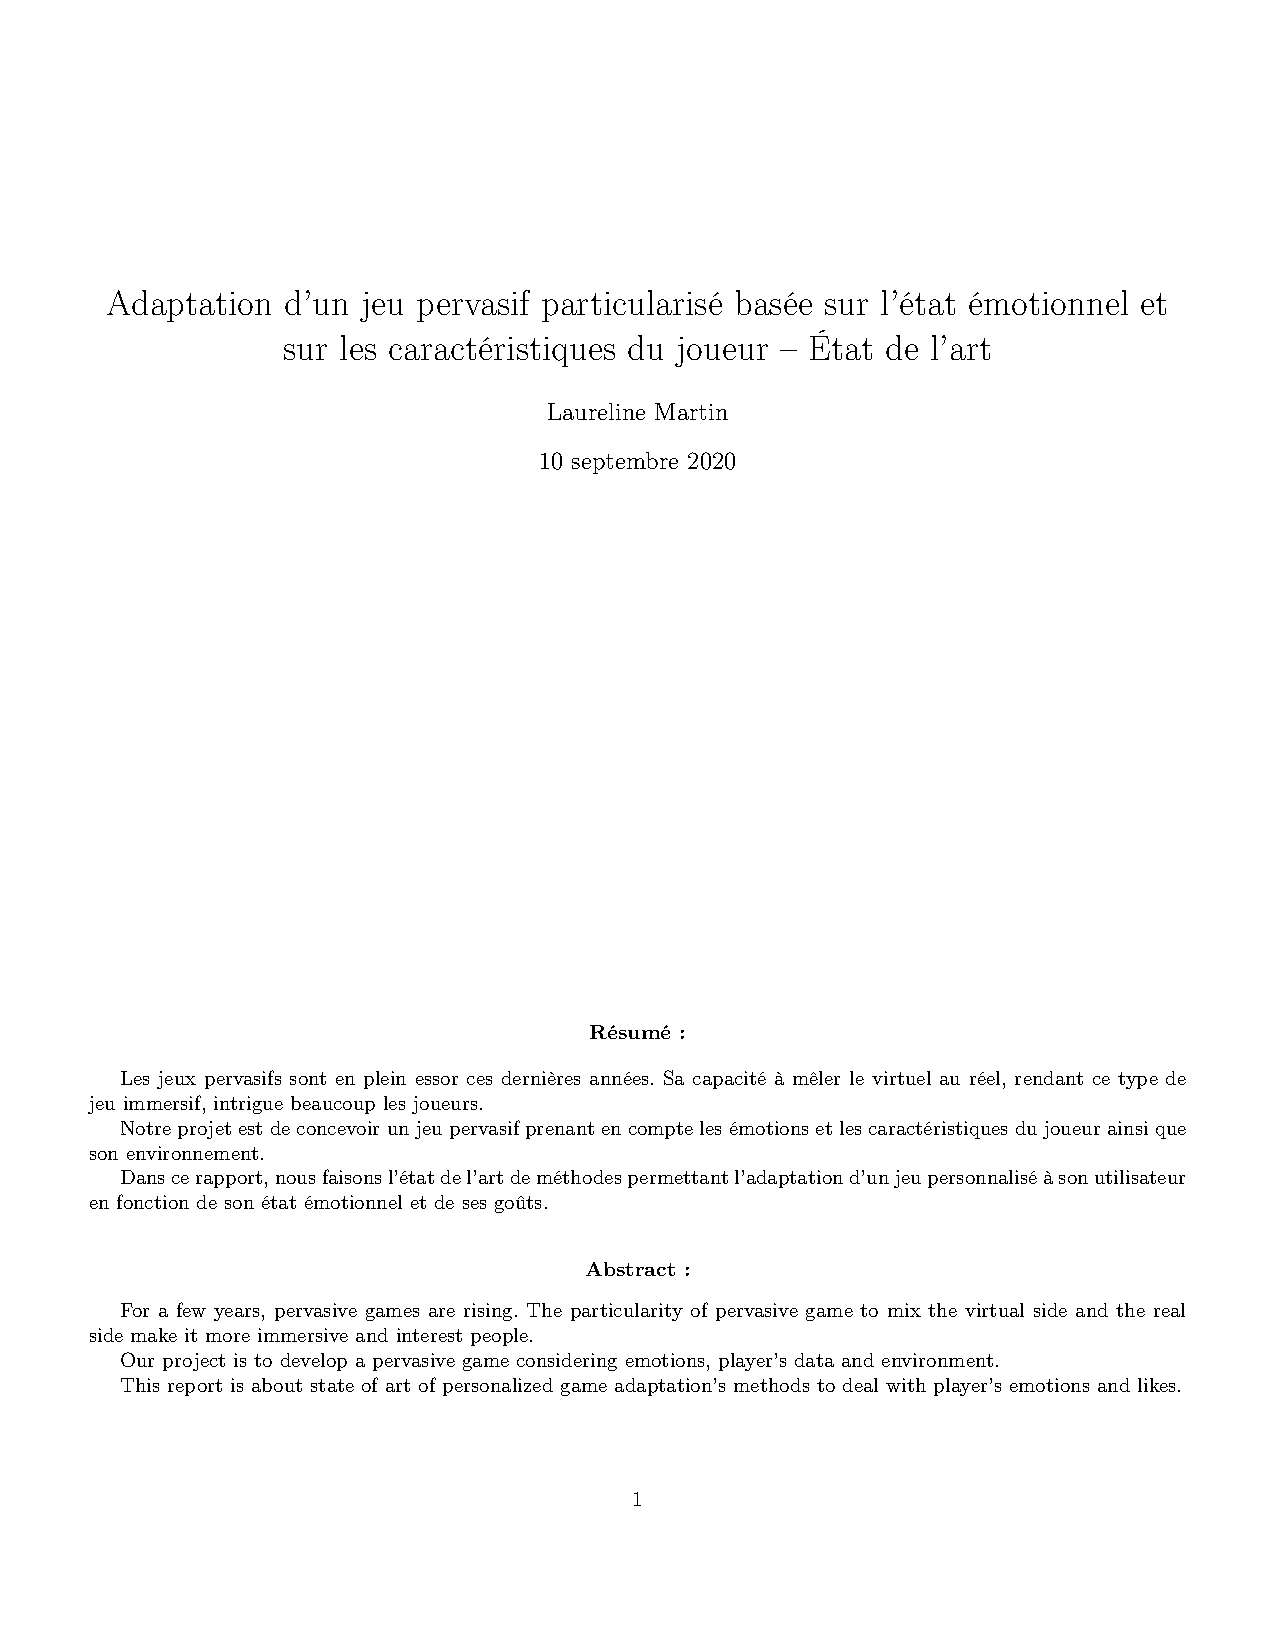
\includepdf[pages=-]{../include/eda.pdf}
		%\makeatletter
		%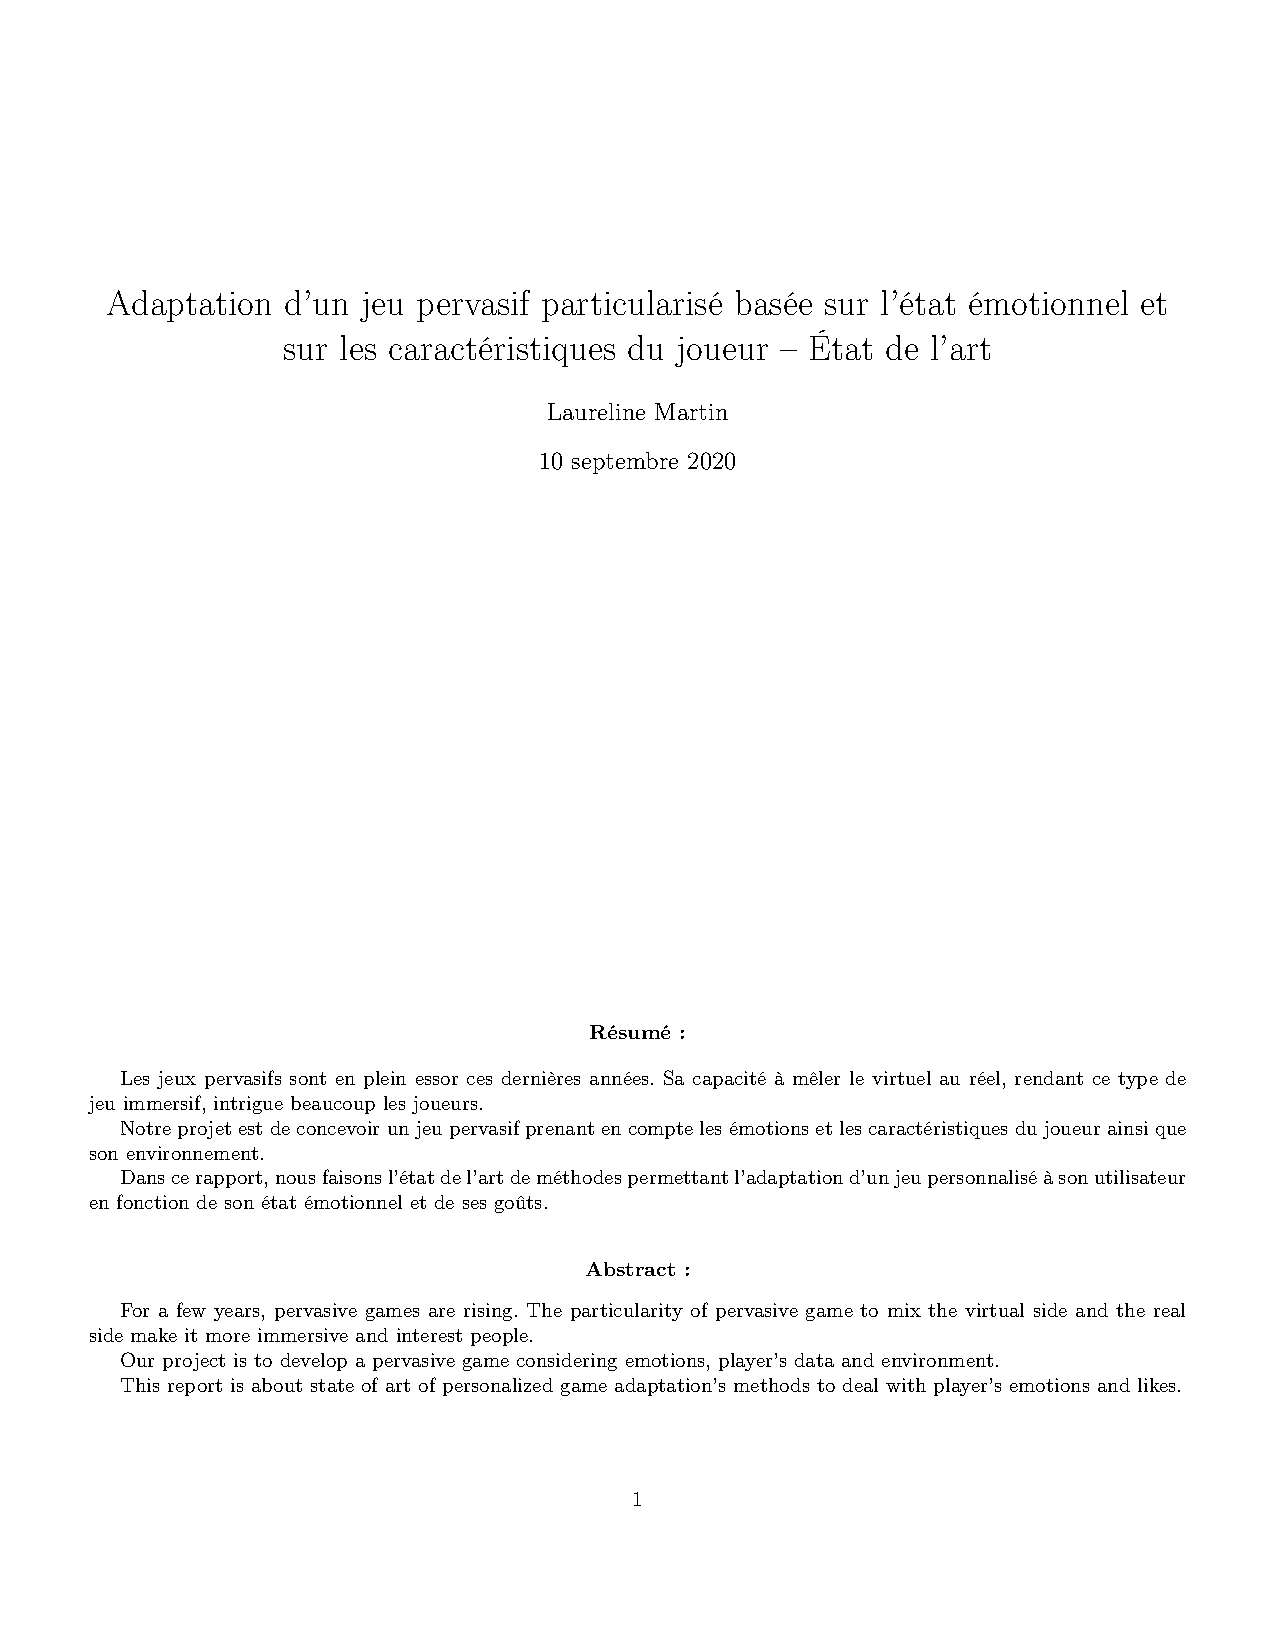
\includepdf[pages=-,picturecommand={%
		%           \setlength{\@tempdimb}{.5\paperwidth}%
		%           \setlength{\@tempdimc}{2cm}%
		%           \setlength{\unitlength}{1pt}%
		%           \put(\strip@pt\@tempdimb,\strip@pt\@tempdimc){%
		%       \makebox (0,0){\thepage}}%
		%}]{../include/eda.pdf}
		%\makeatother
	%\subsection{Lecture de l'état de l'art}
		\subsubsection{Cadre de comparaison}
			Le cadre comparatif $-$pour l'adaptation dynamique de jeux pervasifs aux états émotionnels et à d'autres caractéristiques des joueurs$-$ nous permet d'avoir une vue d'ensemble sur la façon dont l'adaptation est traitée par les méthodes comparées.
			Notre cadre s'appuie sur les critères suivants :
			\begin{itemize}
				\item Les méthodes pour la détection et pour la reconnaissance des états émotionnels
				\begin{itemize}
					\item Les capteurs utilisés
					\item Les algorithmes utlisés pour la détection et/ou la reconnaissance de l'état émotionnel
				\end{itemize}
				\item Les autres caractéristiques de l'utilisateur prises en compte par le jeu
				\item Les méthodes d'adaptation d'un jeu au contexte de son utilisateur
				\begin{itemize}
					\item Méthodes pour l'adaptation du jeu selon l'état émotionnel du joueur
					\item Méthodes pour l'adaptation du jeu selon d'autres caractéristiques du joueur
				\end{itemize}
			\end{itemize}\par
			Le critère "méthodes pour la détection et pour la reconnaissance des états émotionnels" nous permet d'identifier d'une part les capteurs utilisés (s'ils existent).
			Et d'autre part, les algorithmes utilisés pour la détection et la reconnaissance d'états émotionnels.
			Comme nous visons à utiliser des capteurs pour notre projet, il est important pour nous de savoir si certains capteurs reviennent souvent dans la littérature et s'ils sont performants pour ce type d'application.
			Nous visons aussi à utiliser des algorithmes d'apprentissage profond non-supervisés pour la reconnaissance d'états émotionnels (comme celui décrit dans \cite{gal_et_al._2020}), alors nous avons cherché à savoir s'il existait déjà des algorithmes similaires.\par
			Le critère "autres caractéristiques de l'utilisateur prises en compte par le jeu" nous permet d'identifier s'il existe d'autres données que celles concernant l'état émotionnel pour une "bonne" adaptation d'un jeu.
			Ce critère permet d'élargir notre champ de recherche.\par
			Le dernier critère "méthodes d'adaptation d'un jeu au contexte de son utilisateur" permet d'identifier les algorithmes pour l'adaptation dynamique et particularisée d'un jeu.
			D'un côté nous explorons les algorithmes utilisant l'état émotionnel du joueur.
			Et de l'autre, nous explorons les algorithmes utilisant d'autres caractéristiques du joueur.
			Comme nous souhaitons que notre jeu soit particularisé à chaque joueur et que l'adaptation se fasse en temps-réel, nous cherchons des approches qui utilisent ce genre d'algorithmes.
			Nous nous intéressons tout particulièrement aux approches qui présentent des algorithmes pour l'adaptation dynamique aux états émotionnels des joueurs.\par
			Ce cadre peut être appliqué à des recherches scientifiques et à des jeux déjà existants sur le marché.
			Pour notre état de l'art, nous avons appliqué notre cadre à douze approches différentes.
			Ces approches concernent différents types de jeux (jeux sérieux, jeux-vidéo, jeux pervasifs,...).
		\subsubsection{Application du cadre}
			De cette comparaison, il en ressort plusieurs questions et limites.\par
			Tout d'abord, nous remarquons que seulement quelques états émotionnels sont traités dans les approches que nous avons étudiées.
			Même si nous pouvons imaginer que certains états émotionnels ne seront jamais expérimentés au cours du jeu que nous souhaitons concevoir, il semble tout de même important de pouvoir prendre en compte le plus grand nombre d'états émotionnels possible.
			Sans quoi, le jeu ne pourrait pas s'adapter correctement au joueur et impacter négativement son expérience et son niveau d'intérêt pour le jeu.
			Notre idée n'est pas de détecter et de reconnaître tous les états émotionnels.
			Nous souhaitons utiliser un algorithme d'apprentissage profond non-supervisé afin de trouver des motifs particuliers permettant de détecter un changement d'un état émotionnel vers un autre.
			Avec cette information, nous serions en mesure de connaître l'état émotionnel courant du joueur.\par
			Dans notre cas, nous utilisons des capteurs physiologiques de contact, c'est-à-dire des capteurs "collés" au joueur, dans le but d'acquérir des données sur son état physiologique courant pour en déduire son état émotionnel courant via des algorithmes.
			Dans les approches que nous avons relevées, certaines d'entre elles reconnaissent des états émotionnels en utilisant différents types d'algorithmes et des capteurs physiologiques.
			Mais contrairement à cela, d'autres utilisent des modèles pour "prédire" l'état émotionnel courant du joueur.
			Ces méthodes "prédictives" peuvent être intéressantes car elles ne nécessitent pas de capteurs.
			Le joueur n'a pas à acheter des capteurs, ni à les "coller" sur lui pour que le jeu puisse détecter son état émotionnel courant.
			Il est donc "plus libre" dans ses mouvements.
			Cependant, ce type de méthodes semble être moins précis car il se base sur le principe que tous les joueurs ressentiront exactement le même état émotionnel lorsqu'ils se retrouveront dans le même cas de figure.
			De plus, cela implique d'envisager absolument tous les états du jeu possibles, toutes les actions possibles du joueur et d'associer un état émotionnel pour chaque intersection.
			Ceci nous laisse croire que l'utilisation de capteurs physiologiques, même si leur utilisation est plus contraignante pour le joueur, est plus pertinente car plus proche de chacun puisque les capteurs génèrent des données propres à chaque joueur.
			Nous pensons que deux états émotionnels distincts pourront être expérimentés par deux joueurs différents, même s'il s'agit de la même situation dans le jeu pour les deux joueurs.
			De ce fait, il est nécessaire que le jeu s'adapte à chacun dynamiquement.\par
			Notre cadre de comparaison révèle que d'autres caractéristiques que celle de l'état émotionnel peuvent être considérées pour augmenter la "connaissance" du jeu sur son joueur.
			Ces caractéristiques peuvent être intéressantes à étudier à la fois pour mieux connaître les goûts et les préférences du joueur (qui sont souvent plus pérennes) mais aussi pour l'enrichissement de la connaissance du contexte de l'environnement globale.
			Ces caractéristiques peuvent aussi bien s'appuyer sur l'utilisation d'un questionnaire de préférences rempli par l'utilisateur lui-même, que sur la présence de capteurs dans l'environnement.
			Cela constitue une piste qui pourrait être approfondie dans de prochains travaux.\par
			Cet état de l'art nous a permis d'avoir une vision globale de ce qui existait déjà en matière d'adaptation de jeux aux états émotionnels des joueurs. 
			Il nous a permis d'affiner les contours pour la conceptualisation d'un jeu pervasif capable de s'adapter dynamiqument aux états émotionnels de son joueur et de trouver de nouvelles pistes de réflexions. 
			Il a aussi été l'occasion de proposer un cadre de comparaison pour ce sujet.
			Grâce à cet état de l'art, j'ai pu comprendre quels sont les enjeux pour la réalisation de notre objectif.

\section{Expérience d'un escape game}\label{sec:escape}
	Nous avons expérimenté sur nous-mêmes un escape game.
	La salle que nous avons testée se trouve au Victory Escape Game\footnote{\href{http://www.victoryescapegame.fr/}{http://www.victoryescapegame.fr/}} situé au 37 rue des Gravilliers à Paris.
	Cela a été l'occasion d'expérimenter ce genre de jeu très immersif. 
	Dans cette section, nous abordons tout d'abord la notion d'expérience utilisateur.
	Puis, nous faisons un retour sur cette expérience d'escape game et ce qu'elle a pu apporter pour le projet que nous menons.
	\subsection{Expérience Utilisateur}\label{sec:UX}
		L'expérience utilisateur (UX pour User eXperience) est un sujet de psychologie et de neurosciences en perpétuel développement.
		Des méthodes plus efficaces pour donner la meilleure expérience utilisateur sont continuellement recherchées.
		De plus, la connaissance et la compréhension du fonctionnement du cerveau humain est aussi un domaine où l'on fait sans cesse de nouvelles découvertes.
		De ce fait, il n'existe pas de "définition universelle" de l'UX.
		Je présente ici ma propre définition de l'expérience utilisateur.
		Pour construire cette définition, j'ai étudié différentes ressources qui se trouvent en Annexe \ref{ann:ux}.\par
		L’expérience utilisateur concerne toutes les réactions qu’un utilisateur peut avoir lors d’une interaction avec un service, un objet, un espace public, etc.
		C’est aussi tout ce que l’utilisateur peut ressentir lors de cette interaction.
		La notion d’expérience utilisateur va donc plus loin que la simple notion d’ergonomie qui elle ne concerne que la « facilité d’utilisation » d’un produit.\par
		L’UX commence par la perception sensorielle de l’utilisateur de ce qu’il lui est présenté.
		Cette perception est « analysée » par le cerveau et mémorisée.
		Une réaction est ensuite faite (c'est une façon très simplifiée d'expliquer comment cela fonctionne).
		Les concepteurs peuvent alors analyser ces réactions et améliorer leur conception.
		Cette dernière étape est appelée UX Design.
		L’UX Design c’est éprouver un prototype par des utilisateurs de manière itérative.
		Après chaque test utilisateur, le prototype est amélioré et testé à nouveau par des utilisateurs.\par
		L’UX désigne un vaste champ d’application.
		Dès lors qu’une interaction se fait entre un utilisateur et quelque chose, on peut parler d’expérience utilisateur.
		De ce fait, de nombreuses définitions de l’UX existent.
		Chacune d’entre elles tend à s’appliquer d’avantage à un domaine qu’à un autre.
		Dans le cadre de nos recherches, nous traiterons ici, uniquement de l’expérience utilisateur dans les jeux.\par
		Une « bonne » UX vise à maximiser d’une part l’utilisabilité d’un jeu et d’autre part l’engagement du joueur.\par
		L’utilisabilité rassemble toutes les questions qui concernent la facilité de compréhension et d'utilisation du jeu.
		Cela va de la visibilité et de la compréhension des affichages dans le jeu par le joueur à la facilité de faire des actions.
		Par exemple, la souris d’un ordinateur étant généralement à droite, on évitera de demander au joueur à la fois de cliquer sur la souris et d’appuyer sur des touches situées sur la droite du clavier.
		En UX design, il existe des cadres et des règles à appliquer pour une bonne utilisabilité d’un jeu.\par
		L’engagement (i.e. le flow ou l’immersion) concerne la partie « émotionnelle » de l’interaction entre le joueur et le jeu.
		Il s’agit de réussir à motiver le joueur à commencer ou à continuer à jouer.
		Cela peut se faire par l’accomplissement d’objectifs pour obtenir des récompenses.
		La progression, la coopération, la compétition, etc. sont également des éléments motivants pour le joueur.
		Créer des émotions au joueur tout au long de sa partie permet également un meilleur engagement.
		De plus, il faut que la difficulté du jeu soit bien « réglée » pour que le joueur n’ait ni une sensation d’ennui ni envie de rejeter le jeu.
		Cela peut passer par exemple, par l’apprentissage du jeu via des tutoriels.
	\subsection{Expérimentation d'un escape game}\label{sec:expescape}
		L'escape game que nous avons expérimenté se présentait sous la forme d'une mission d'une heure.
		Le but de cette mission était d'entrer dans un vaisseau désaffecté pour emprunter un portail de téléportation.
		Celui-ci étant cassé, il fallait récupérer des indices dissimulés dans les pièces pour le redémarrer.\par
		Tout d'abord, nous avons été sensibilisés à la mission qui nous attendait par le maître du jeu.
		Il s'agissait d'une réunion d'une vingtaine de minutes pour nous expliquer d'une part les règles mais aussi notre objectif.
		Cette sensibilisation est un premier contact indirect avec le jeu et me semble tout aussi importante que le jeu en lui-même.
		C'est une méthode pour nous motiver à jouer et à être performant dans notre jeu.
		Un sentiment de compétition a aussi été implicitement donné lorsque le maître du jeu nous a indiqué les meilleurs temps d'autres joueurs.\par
		Le principe de l'escape game est de fouiller les pièces pour trouver des indices pour débloquer des mécanismes et rejoindre la sortie.
		Les indices étaient de toutes sortes : écrits, lumineux, objets, boutons poussoirs, textiles, etc.
		Il pouvait aussi se trouver de faux indices.
		Les pièces ont été décorées, pour donner l'impression d'un vaisseau spatial.
		Le but est de donner la sensation la plus forte possible au joueur qu'il se trouve dans un "véritable" vaisseau dans l'espace.\par
		Pendant cette partie, le maître du jeu $-$qui se trouvait dans une autre pièce et qui nous observait grâce à des caméras et des micros$-$ pouvait nous donner des indices supplémentaires aux indices déjà présents dans la pièce via à un écran.
		Un message nous donnant un indice sur le mécanisme à débloquer appariassait accompagné d'un indicateur sonore.
		Les messages que nous recevions par cet écran faisaient penser qu'il s'agissait d'indications données par une intelligence artificielle.\par
		Tous les objets et le décor des différentes pièces permettent de créer une ambiance et plonger immédiatement les joueurs dans l'univers où les créateurs du jeu essayent de les emmener.
		Nous avons pu également relever quelques méthodes d'UX design comme l'utilisation d'objectifs à atteindre.
		Par exemple, l'objectif principal est de sortir du vaisseau avant le temps imparti (une heure) et pour y parvenir, il faut réussir à ouvrir différentes portes pour accéder aux pièces suivantes.
		L'utilisation d'un compte-à-rebours affiché en permanence à l'écran créait un sentiment de stress.
		Chaque alerte sonore indiquant qu'un nouveau mécanisme avait été débloqué donné un sentiment de satisfaction.\par
		Nous n'avons pas réussi à arriver jusqu'au bout de notre "mission". Cinq minutes avant la fin du compte-à-rebours nous sommes arrivés à la dernière salle.
		Nous ne nous attendions pas à cette dernière salle et avons été très surpris.
		Cela a été un peu frustrant de ne pas pouvoir terminer cette session avant la fin du compte-à-rebours.
	\subsection{Accessibilité d'un escape game}
		Dans cette partie, je vais aborder les limites de l'accessibilité aux déficients visuels de l'escape game et généraliser aux jeux.
		Il s'agit d'un témoignage et non d'une recherche à part entière.
		Ce témoignage pourra nous donner une piste de réflexion pour notre propre jeu pervasif.\par
		Etant personnellement déficiente visuelle, je vais vous rapporter mon expérience personnelle de l'escape game que nous avons expérimenté.\par
		Pour atteindre l'objectif qui était de réparer portail de téléportation, il fallait rechercher dans différentes pièces des indices.
		Le premier obstacle rencontré lors cette partie était celui du déchiffrage des indices.
		En effet, beaucoup d'indices se basenu sur de l'écriture et sur d'autres mécanismes très visuels.
		Par exemple, nous avions trouvé un dossier contenant plusieurs pages écrites avec une taille de police standard (comme celle de ce rapport par exemple).
		Cet indice m'était donc inaccessible, je distinguais seulement quelques logos qui se trouvaient dans ce dossier.
		Un autre élément inaccessible pour moi était une grande carte affichée dans une des pièces où il fallait retrouver des coordonnées et ajuster des boutons par rapport à ces coordonnées.
		Ce type d'élément m'était complètement inaccessible car il s'appuie uniquement sur la capacité du joueur à repérer des éléments visuels parmi un tas d'autres informations visuelles entremêlées.
		J'ai aussi rencontré des difficultés dues à la luminosité basse des pièces.
		De plus, avec la situation sanitaire actuelle, nous étions obligés de porter des gants pour jouer puisqu'il fallait toucher et prendre beaucoup d'objets.
		Cependant, porter des gants empêche de sentir beaucoup de choses et m'a privé d'informations par le touché que d'autres ont par le visuel.\par
		Toutes ces limites m'ont fait sortir du jeu et casser le rythme et l'intrigue.
		De ce point de vue, je peux dire que mon expérience utilisateur à été moyenne.
		J'ai été "déconnectée" de certains indices et j'ai dû laissé mes coéquipiers prendre le relais sur ce que ne je pouvais pas voir.
		Ce qui a probablement joué sur leur expérience utilisateur également.
	\subsection{Bilan}\label{sec:escapebilan}
		Nous retenons plusieurs points de cette expérimentation.
		Cet escape game nous a permis d'appliquer à nous-mêmes le ressenti de joueurs.
		Cela nous a permis de rappeler ce qu'était l'expérience utilisateur et à quoi cela pouvait servir pour améliorer un jeu.
		Nous avons pu expérimenter différents états émotionnels lors de cette session.
		Le fait d'avoir ressenti différents états émotionnels et d'avoir été motivés durant toute la partie à jouer montre que l'UX design est important pour le joueur, pour son expérience de jeu et pour son amusement.\par
		Nous avons pu constater que beaucoup de méthodes issues de l'UX Design étaient appliquées à l'escape game que nous avons expérimenté.
		Comme la sensibilisation, le décor, la motivation, la coopération, les émotions, l'affichage de compte-à-rebours et d'indications.
		Ce sont autant de méthodes qui ont été mise en place pour améliorer l'expérience du joueur.
		La salle que nous avons expérimentée a été testée et améliorée plusieurs fois avant d'être proposée aux joueurs.
		De plus, elle est encore améliorée selon les retours qui sont fait par les joueurs si les créateurs jugent cela pertinent.
		Cela est fait pour tendre à la meilleure UX possible pour cette salle.\par
		Cette expérience d'escape game et mon expérience personnelle m'a fait comprendre l'importance de mener des expérimentation "en réel".
		Bien souvent, les expériences sont menées en laboratoire.
		Comme celles décrites dans les références présentées dans l'état de l'art à la Section \ref{sec:eda} ou celles menées pour améliorer l'UX.
		Nous remarquons que bien souvent, ces expériences n'impliquent que des personnes n'ayant aucun problème de santé, dans une fourchette d'âge restreinte, etc.
		Cette méthode d'expérimentation exclue certains joueurs et crée un décalage entre les testeurs du jeu et le public réel.
		D'après toutes ces remarques, il me semble important d'ouvrir le groupe test au public le plus large possible.
		Autrement dit, d'étendre les âges, les cultures, les capacités physiques, etc. le plus possible afin de permettre une plus grande inclusivité.\par
		Mon expérience personnelle par rapport à cet escape game montre plusieurs limites d'accessibilité pour ce type de jeu.
		D'après cette expérience, je pense qu'il faut rendre d'avantage les jeux accessibles à tous les publics.
		Pour cela, une idée serait de rentre les jeux plus adaptables et personnalisables.
		Dans le jeu pervasif, les défis pour une meilleure accessibilité du jeu sont multiples.
		On peut par exemple penser à l'interface utilsateur qui doit être accessibles au personnes daltoniennes ou déficientes visuelles, ou aux sons émis par le jeu ou par l'environnement qui doivent être traduit pour les personnens mal-entendantes.
		Bien sûr, beaucoup d'autres exemples sont existent.
		Il faut donc que le jeu puisse connaître les difficultés du joueur pour s'y adapter.
		Cependant, on peut imaginer que rendre le jeu "trop" adaptable pourrait dégrader l'expérience du joueur.
		Si le jeu s'adapte mal au joueur, son expérience pourrait être moins bonne.
		Ou bien, si l'adaptatino du jeu supprime certains aspect ou certaines 
		Il faudrait donc chercher un bon équilibre entre adaptabilité, jouabilité et expérience utilisateur.\par
		Nous pouvons envisager de réitérer ce genre d'expérimentations pour approfondir les sujets de l'expérience utilisateur dans les jeux immersifs et des états émotionnels ressentis lors d'une partie d'escape game.
		Nous pouvons aussi imaginer utiliser nos capteurs lors de prochaines parties et d'en analyser les données pour essayer de déterminer des changements d'états émotionnels significatifs qui correspondraient à des événements lors de la parite (indice découvert, porte débloquée,...).

\section{Modélisation conceptuelle}\label{sec:modelisation}
	Dans cette partie, nous présentons un modèle conceptuel qui est en cours d'aboutissement.
	Le but de ce modèle conceptuel est de représenter chaque composant permettant la prise en compte des états émotionnels dans le jeu pervasif et de s'y adapter.
	Le modèle doit à la fois représenter le joueur, le jeu, les états émotionnels, les capteurs mais aussi des composants plus abstraits comme les réactions physiologiques du joueur, la reconnaissance des états émotionnels, l'adaptation dynamique du jeu, etc.
	Cette représentation est modélisée sous la forme d'une ontologie.
	Pour cela, nous utilisons le format standard du diagramme de classes UML.
	\subsection{Ontologie}\label{sec:ontologie}
		\begin{figure}[t]
			\centering
			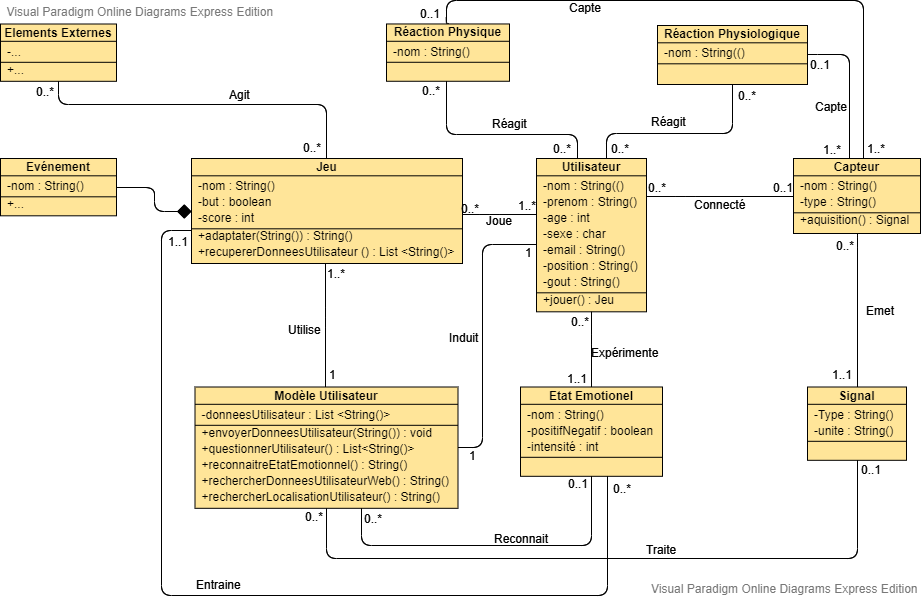
\includegraphics[scale=0.5]{../include/ontologie_stage_cnam-v2-5.png}
			\caption{Ontologie d'un jeu pervasif prenant en compte l'état émotionnel du joueur}
			\label{fig:modele}
		\end{figure}
		Le diagramme de la Figure \ref{fig:modele} représente notre modélisation pour les différents éléments qui composent un jeu pervasif adaptable aux états émotionnels du joueur.
		Pour chaque classe, il existe une description détaillée en Annexe \ref{ann:detailclasses}.\par
		Nous pouvons relever plusieurs défauts à ce modèle que nous pourrions améliorer.
		Par exemple, il existe dans ce modèle une relation entre les classes \texttt{Utilisateur}, \texttt{Jeu} et \texttt{Etat Emotionnel} que j'aurais pu représenter par une relation ternaire.
		Cependant, j'ai préféré décomposer cette relation en trois relations binaires dans un soucis de clarté.
		Une amélioration possible pour cette représentation est celle de la relation entre \texttt{Jeu} et \texttt{Modèle Utilisateur}.
		Avec du recul sur mon travail, je pense qu'il aurait été possible de soit fusionner les deux classes (puisqu'il s'agit d'une relation $1^* - 1$) soit de transformer la classe \texttt{Modèle Utilisateur} en une ou plusieurs autre(s) classe(s).
		De la même manière, la classe \texttt{Signal} ne devrait pas figurer sur ce modèle.
		Selon moi, il faudrait inclure la classe \texttt{Signal} dans la classe \texttt{Capteur}.
		Bien d'autres améliorations sont envisageables pour ce modèle.
	\subsection{Difficultés rencontrées}\label{sec:difficultes}
		L'ontologie que je présente dans ce rapport à la Figure \ref{fig:modele} n'est pas le résultat définitif du modèle conceptuel que nous cherchons à élaborer.
		Lors de l'élaboration de cette cette ontologie, plusieurs essais et plusieurs versions différentes ont été proposés.
		Cependant, le modèle était toujours incohérent, il manquait de substance et présentait plusieurs niveaux d'abstraction qui ne devait pas figurer sur un même modèle. 
		Cela peut s'expliquer de différentes manières. 
		L'une des explications est que je me suis lancée trop rapidement, selon moi, dans la conception de cette ontologie.
		Je pense que je ne maîtrisais pas encore assez bien le sujet, l'objectif et la problématique de notre projet.
		De ce fait, j'ai eu tendance à mélanger les niveaux d'abstraction.
		Une autre explication est qu'avec les différentes approches que je lisais parallèlement à la construction de cette ontologie, j'ai voulu retranscrire dans ce modèle tout ce que j'assimilais au fil de mes lectures.
		Ce qui faisait que j'ajoutais à ce modèle des éléments superflus.
		Une dernière explication est que je manquais de recul sur mon travail.
		Dès que je terminais une version de l'ontologie et que celle-ci n'était pas correcte, je commençait une nouvelle version.
		Je ne laissais pas de temps de repos entre chaque nouvel essai.\par
		C'est pour toutes ces raisons que nous avons décidé de changer de point de vue et de problématique.
		Nous avons décidé de revenir, si possible, plus tard à l'ontologie.
	\subsection{Bilan}\label{sec:modelbilan}
		Le bilan que je tire de cet exercice de modélisation est que malgré cet échec d'aboutir à une ontologie livrable, j'ai pu, d'une part, mieux comprendre la problématique liée au projet et à la conception de modèles.
		Et d'autre part, j'ai pu me rendre compte de l'étendue des difficultés qu'il  était possible de rencontrer dans ce genre d'exercice.
		Par exemple, lors de la conception de cette ontologie, je me suis retrouvée à mélanger plusieurs niveaux d'abstraction, ce qui la rendait peu compréhensible et invalide.
		Je me suis aussi rendu compte qu'il fallait beaucoup de patience et d'entraînement pour concevoir un tel modèle.
		Aujourd'hui, je comprends mieux les enjeux de tels modèles.
		A l'avenir je pourrais réaliser des modèles de meilleure qualité grâce à cette expérience.\par
		La réalisation de cette ontologie nous a permis de réorienter notre objectif de recherche.
		Nous nous sommes dirigés vers l'implémentation d'une solution pour la gestion des données générées par les capteurs physiologiques.

\section{Prototypage}\label{sec:prototypage}
	Pour la détection et la reconnaissance de l'état émotionnel dans le jeu pervasif que nous souhaitons réaliser, des  capteurs physiologiques de contacts sont utilisés.
	Ces capteurs prennent des mesures en continu pour différentes métriques physiologiques telles que la température du corps, le rythme cardiaque, la réponse électrodermale ou encore la fréquence respiratoire.
	Ces capteurs génèrent beaucoup de données.
	De plus, il s'agit de données en temps-réel qui doivent être traitées le plus rapidement possible pour reconnaître l'état émotionnel courant d'une personne. 
	Ainsi, le jeu pourra s'adapter à son utilisateur avec un minimum de latence. 
	Une trop grande latence pourrait engendrer un effet de décalage désagréable pour le joueur entre ce qu'il ressent et l'adaptation du jeu.\par
	Dans cette section, nous présentons une solution pour la gestion de telles données. 
	Pour construire cette solution, nous avons tout d'abord comparé deux technologies et nous nous sommes positionnés sur l'une d'entre elles.
	Puis, nous avons implémenté un prototype de cette solution.
	Nous présentons son architecture globale.
	Enfin, nous expliquons comment cette contribution peut être intégrée aux travaux déjà menés pour notre projet.
	\subsection{Technologie utilisée}\label{sec:prototech}
		Pour notre prototype, nous avons besoin d'ingérer le plus rapidement possible des données en temps-réel qui sont générées toutes les 30 à 60 millisecondes.
		Il nous faut donc trouver une technologie capable de traiter efficacement ce genre de données pour les transmettre aux algorithmes de détection et de reconnaissance de l'état émotionnel.
		Autrement dit, notre solution doit être capable de "faire le lien" entre les capteurs physiologiques et les algorithmes de détection et de reconnaissance d'états émotionnels.\par
		Pour cela, nous avons comparé deux Middleware Orientés Messages et nous en avons retenu un pour concevoir notre solution.
		\subsubsection{Comparaison entre Apache Kafka et RabbitMQ}\label{sec:comparatif}
			Notre choix s'est porté sur les Middleware Orientés Messages (MOM).
			Ces middleware ont pour objectif de transmettre un message d'un utilisateur à un autre.\par
			Nous avons sélectionné deux middleware libres, simples d'utilisation et avec une communauté active.
			Il s'agit d'Apache Kafka et de RabbitMQ.
			Avant de commencer la synthèse comparative entre ces deux middleware,  introduisons les points communs entre Apache Kafka et RabbitMQ :
			\begin{itemize}
				\item Ce sont deux Middleware Orienté Message (MOM);
				\item Ils ont le même ordre de grandeur de messages consommables par seconde (un peu plus du côté Kafka);
				\item Ils sont Open Source.
			\end{itemize}
			Apache Kafka et RabbitMQ sont utilisables dans les domaines d'application suivants :
			\begin{itemize}
				\item Collecter de l’information pour l'Internet des Objets (IoT);
				\item Transmettre des métriques;
				\item Envoyer des notifications, des mails, des messages instantanées,...;
				\item Transmettre des actions utilisateurs;
				\item Faire des actions compte bancaire à compte bancaire (i.e. des transactions).
			\end{itemize}\par
			Maintenant que nous connaissons les points communs entre les deux MOM, nous pouvons en faire une comparaison synthétique.\par
			Dans ce comparatif, nous traitons des principales différences des deux middleware dans le Tableau \ref{tab:comparatifinfos}, de leurs architectures dans le Tableau \ref{tab:comparatifarchi} et dans la Figure \ref{fig:comparatifarchi}, de leurs approches dans le Tableau \ref{tab:comparatifapp}, des caractéristiques des messages dans le Tableau \ref{tab:comparatifmess} et de la préférence d'utilisation de l'un ou de l'autre MOM selon le cas d'usage dans le Tableau \ref{tab:comparatifpref}.\par
			\begin{table}
				\begin{tabular}{|p{7.5cm}|p{7.5cm}|}
					\hline
					\rowcolor{lightgray} RabbitMQ & Kafka\\\hline
					Depuis 2007 & Depuis 2011\\\hline
					Destiné au début : en tant que composante primaire dans les messageries SOA ;\newline Maintenant : pour le flux de données & Pour le scenario de flux\\\hline
					Structure de données : FIFO;\newline Optimal quand les messages sont livrés rapidement & Structure de données : Log (le consommateur gère l’offset);\newline Possibilité de relire des données, les messages sont conservés selon un temps paramétré\\\hline
					Inclus les protocoles : MQTT, AMQP, STQMP;\newline Facilité la communication avec d’autres solutions implémentant AMQP & Routage simple (clé de routage);\newline Les messages sont sur des « topics » (les consommateurs s’abonnent aux topics voulus)\\\hline
					Mode de délivrance des messages : \textit{at least once} & Modes de délivrance des messages : \textit{at least once} et \textit{exactly once}\\\hline
				\end{tabular}
				\caption{Principales différences / informations générales des deux MOM}
				\label{tab:comparatifinfos}
			\end{table}
			\medskip
			\begin{table}
				\begin{tabular}{|p{3cm}|p{6cm}|p{6cm}|}
					\hline
					\rowcolor{lightgray} & RabbitMQ & Kafka\\\hline
					Stocakge & Dans une base Mnésia.\newline Qand il y a saturation sur la base Mnésia, le stockage se fait sur disque & Sur disque, dans des fichiers (tailles équiv.), logs. Cluster de servers, dans des topics (durable)\\\hline
					Modèle d'intégration & Point-to-point & Publish / Subscribe\\\hline
					Routage & Flexible & Basique\\\hline
					Structure de données & File FIFO & Log\\\hline
				\end{tabular}
				\caption{Architectures}
				\label{tab:comparatifarchi}
			\end{table}
			\medskip
			\begin{figure}
				\begin{subfigure}{0.6\textwidth}
					\hspace*{-2cm}
					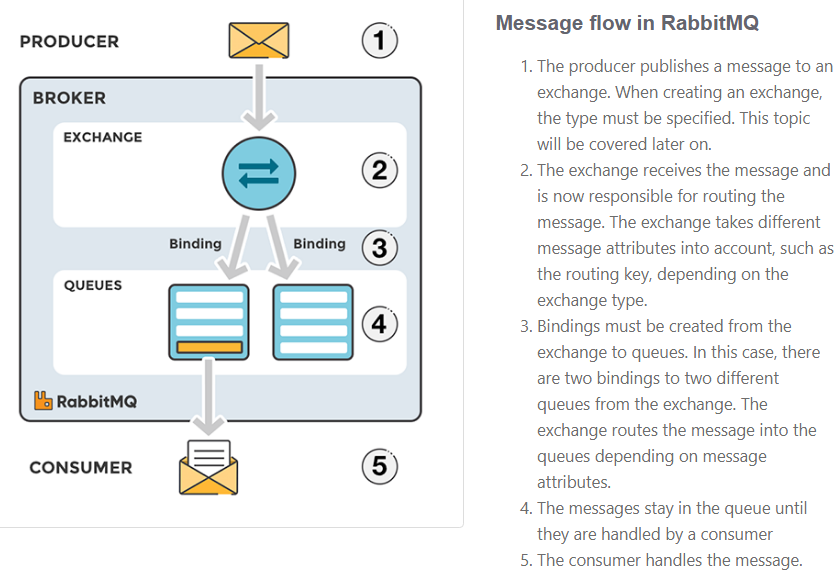
\includegraphics[scale=0.5]{../include/RabbitMQ.PNG}
					\caption{Schéma de l'architecture de RabbitMQ\footnote{\href{https://www.cloudamqp.com/blog/2015-05-18-part1-rabbitmq-for-beginners-what-is-rabbitmq.html}{https://www.cloudamqp.com/blog/2015-05-18-part1-rabbitmq-for-beginners-what-is-rabbitmq.html} (consulté le 28/08/20)}}
					\label{fig:archirabbitmq}
				\end{subfigure}
				\begin{subfigure}{0.5\textwidth}
					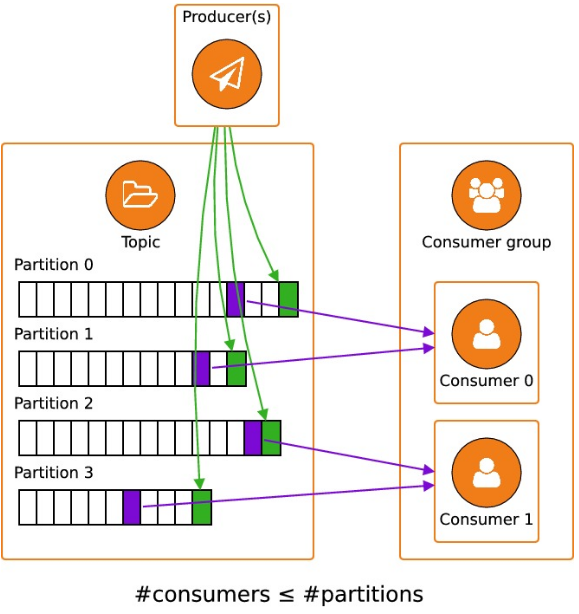
\includegraphics[scale=0.55]{../include/Kafka.PNG}
					\caption{Schéma de l'architecture de Kafka\footnote{\href{https://openclassrooms.com/fr/courses/4451251-gerez-des-flux-de-donnees-temps-reel/4451521-metamorphosez-vos-applications-temps-reel-avec-kafka}{https://openclassrooms.com/fr/courses/4451251-gerez-des-flux-de-donnees-temps-reel/4451521-metamorphosez-vos-applications-temps-reel-avec-kafka} (consulté le 28/08/20)}}
					\label{fig:archikafka}
				\end{subfigure}
				\caption{Schémas des architectures}
				\label{fig:comparatifarchi}
			\end{figure}
			\medskip
			\begin{table}
				\begin{tabular}{|p{7.5cm}|p{7.5cm}|}
				\hline
				\rowcolor{lightgray} RabbitMQ & Kafka\\\hline
				\begin{center} \textbf{Approche Push-based :}\end{center} & \begin{center} \textbf{Approche Pull-based :}\end{center}\\\hline
				Distribuer les messages individuellement et rapidement & Le consommateur récupère les lots souhaités à partir d’un offset spécifique;\newline Mise en commun longue durée\\\hline
				\end{tabular}
				\caption{Approches}
				\label{tab:comparatifapp}
			\end{table}
			\medskip
			\begin{table}
				\begin{tabular}{|p{3cm}|p{6cm}|p{6cm}|}
					\hline
					\rowcolor{lightgray} & RabbitMQ & Kafka\\\hline
					Maintien de l'ordre & Dans une même chaîne (TCP multiplexé) & Dans une même partition\\\hline
					Temps de vie & Jusqu’à que le message soit consommé et l'accusé de réception du consommateur reçu & Délai paramétré (ou si saturation atteinte)\\\hline
					Priorités & Possibilité de définir un degré de priorité des messages & Pas de priorité des messages \\\hline
				\end{tabular}
				\caption{Structure des messages}
				\label{tab:comparatifmess}
			\end{table}
			\medskip
			\begin{table}
				\begin{tabular}{|p{7.5cm}|p{7.5cm}|}
				\hline
				\rowcolor{lightgray} RabbitMQ & Kafka\\\hline
				Besoin de routages élaborés;\newline Utiliser des protocoles STOMP, MQTT ou AMQP...;\newline Suivi de métriques opérationnelles & Besoin en routages simples;\newline Conserver (pour un temps donné) et relire des messages;\newline Mise à l’échelle;\newline Capture d’évènements induisant un changement d’état (dans une base de données ou autre);\newline Besoins transactionnels;\newline Traiter les données en parallèle\\\hline
				\end{tabular}
				\caption{A utiliser de préférence selon le cas d'utilisation}
				\label{tab:comparatifpref}
			\end{table}
			La sitographie sur laquelle je me suis appuyée pour la construction de cette synthèse comparative se trouve en Annexe \ref{ann:kafkarabbitmq}.
		\subsubsection{Positionnement}\label{sec:position}
			Après mes recherches et la rédaction de la synthèse comparative, j'ai décidé d'utiliser Apache Kafka comme Middleware Orienté Message pour le prototypage de notre solution.\par
			Apache Kafka m'a semblé être plus indiqué dans le traitement des données venant de capteurs.
			Ce middleware présente une structure pour les messages en log.
			Ce qui est plus intéressant pour notre cas qu'une structure FIFO (First In, First Out).
			En effet, la structure FIFO nous "oblige" à récupérer et à consommer les messages rapidement dans la queue des messages.
			Tandis qu'une structure en log nous laisse plus de temps et nous permet de relire le message plusieurs fois.
			Ce qui correspond plus à ce que nous cherchons puisque nous n'allons pas consommer toutes les données pour reconnaître un état émotionnel, mais seulement à certains moments (lorsqu'un changement significatif sera détecté). 
			De plus, les données sont organisées dans des "topics". 
			Il est donc possible de récupérer que certaines données en s'abonnant aux topics désirés.
			Autrement dit, en utilisant des topics pour organiser et dissocier les données provenant de différents capteurs, il est possible de ne recupérer que les données provenant de capteurs voulus.
			Cela nous sera très utile pour de futurs travaux qui impliqueront d'autres capteurs que les capteurs physiologiques pour la reconnaissance des états émotionnels.
			Par exemple, nous aurons besoin de capteurs de position, de capteurs placés dans l'environnement du jeu, etc.
			Comme nous souhaitons utiliser différents capteurs pour la détection et la reconnaissance des états émotionnels, les données générés par ces capteurs pourraient être hétérogènes. 
			Apache Kafka propose une API appelé ConnectAPI, qui permet de récupérer des données provenant de sources externes pour les formaliser au format Kafka.
			Cet outil pourra nous servir à homogénéiser les données.
	\subsection{Description du prototype}\label{sec:protodesc}
		Dans cette partie, nous présentons le prototype de la solution que j'ai implémentée pour répondre aux besoins de gestion des données en temps-réel.
		Ici, nous cherchons à gérer au mieux les données en temps-réel en créant un minimum de latence entre la mesure faite par le(s) capteur(s) et la reconnaissance de l'état émotionnel.
		Pour cela, j'ai mis au point une solution qui récupère des données provenant de capteurs physiologiques et qui les distribue sur des topics afin que ces données puissent être consommées par les algorithmes de détection et de reconnaissance d'états émotionnels.\par
		Pour ce prototype, j'ai utilisé un fichier au format CSV contenant plus de 11 000 entrées. 
		Ces entrées concernent des mesures faites lors d'une expérience avec les capteurs décrits dans la Section \ref{sec:capteurs}.
		Cinq métriques ont été captées : le temps (date et heure de l'acquisition), la fréquence cardiaque, la réponse électrodermale, la température à la surface de la peau et le rythme cardiaque.
		Ces entrées sont séparées chacune d'environ 30ms (milisecondes).
		Lors de l'utilisation du Producteur, l'envoie des données dans les topics se fait toutes les 30ms.
		Ce fichier à permis d'éprouver notre protoype.
		A terme, nous souhaitons utiliser uniquement les capteurs comme sources de données en temps-réel et non un fichier contenant des données provenant de capteurs.
		\subsubsection{Architecture du prototype}\label{sec:protoarchi}
			\begin{figure}
				\centering
				\rotatebox{90}{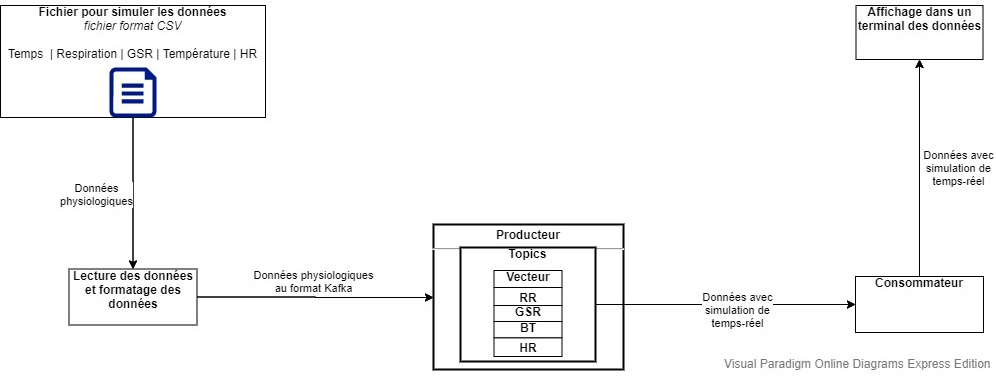
\includegraphics[scale=0.8]{../include/schema-synt-prototype.jpg}}
				\caption{Schéma synthétique de l'architecture du prototype}
				\label{fig:archiproto}
			\end{figure}
			La Figure \ref{fig:archiproto} montre l'architecture de notre prototype.\par
			Pour le moment, nous utilisons un fichier dans lequel se trouve les données provenant de plusierus capteurs.
			Ces données, que nous utilisons pour nos tests, ont été acquises lors d'une session de jeu vidéo à partir de capteurs physiologiques (les capteurs sont décrits dans la Section \ref{sec:capteurs}). 
			Elles ont été enregistrées dans un fichier au format CSV.\par
			Les données sont lues puis envoyées au Producteur.
			Le Producteur ajoute à chaque topic la ou les données qui correspondent.
			Par exemple, les données qui correspondent au Rythme Cardiaque sont envoyées sur le topic "HR" (pour Heart Rate).\par
			Les données peuvent ensuite être consommées par un Consommateur qui choisit le topic auquel il s'abonne.
			Les données sont affichées dans un terminal par le Consommateur au fur et à mesure qu'elles sont produites.
			Le Consommateur attend toujours de nouvelles données à consommer.
		\subsubsection{Implémentation du prototype}
			\begin{figure}[p]
				\centering
				\begin{subfigure}{0.5\textwidth}
					\hspace*{-1cm}
					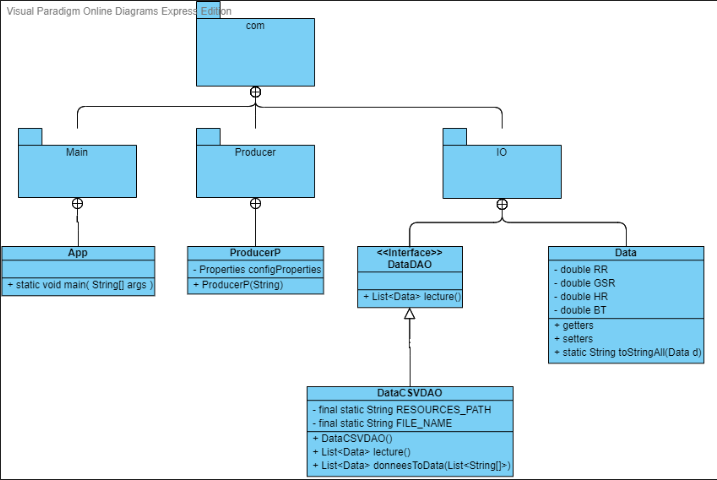
\includegraphics[scale=0.65]{../include/archiProducer.PNG}
					\caption{Architecture du Producteur}
					\label{fig:archiproducer}
				\end{subfigure}\newline
				\begin{subfigure}{0.5\textwidth}
					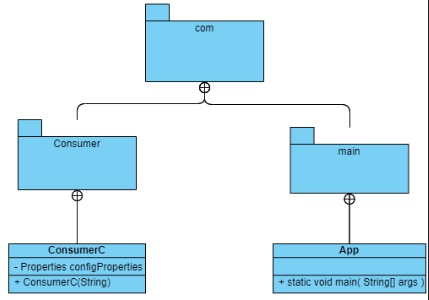
\includegraphics[scale=0.8]{../include/archiConsumer.PNG}
					\caption{Architecture du Consommateur}
					\label{fig:archiconsumer}
				\end{subfigure}
				\caption{Architecture du prototype}
				\label{fig:archiimp}
			\end{figure}
			La Figure \ref{fig:archiimp} décrit les différents composants qui sont utilisés pour l'implémentation de notre prototype.\par
			Le prototype est divisé en deux :
			la partie Producteur (sur la Figure \ref{fig:archiproducer}) et la partie Consommateur (sur la Figure \ref{fig:archiconsumer}). 
			Il s'agit de deux projets \texttt{Maven} distincts qui génèrent chacun un JAR exectuable.\par
			La partie Producteur contient un lecteur de fichiers qui permet de lire les données des capteurs physiologiques contenues dans le fichier \texttt{data\_file.csv}. 
			Ces données sont normalisées grâce à l'objet \texttt{Data} pour être utilisées par le Producteur.
			Le Producteur lit chaque donnée et l'envoie sur un topic.
			Il s'arrête lorsque toutes les données ont été envoyées.\par
			La partie Consommateur "écoute" le topic qui lui est passé en argument et affiche chaque donnée de ce topic dans un terminal.\par
			\begin{figure}
				\hspace*{-0.7cm}
				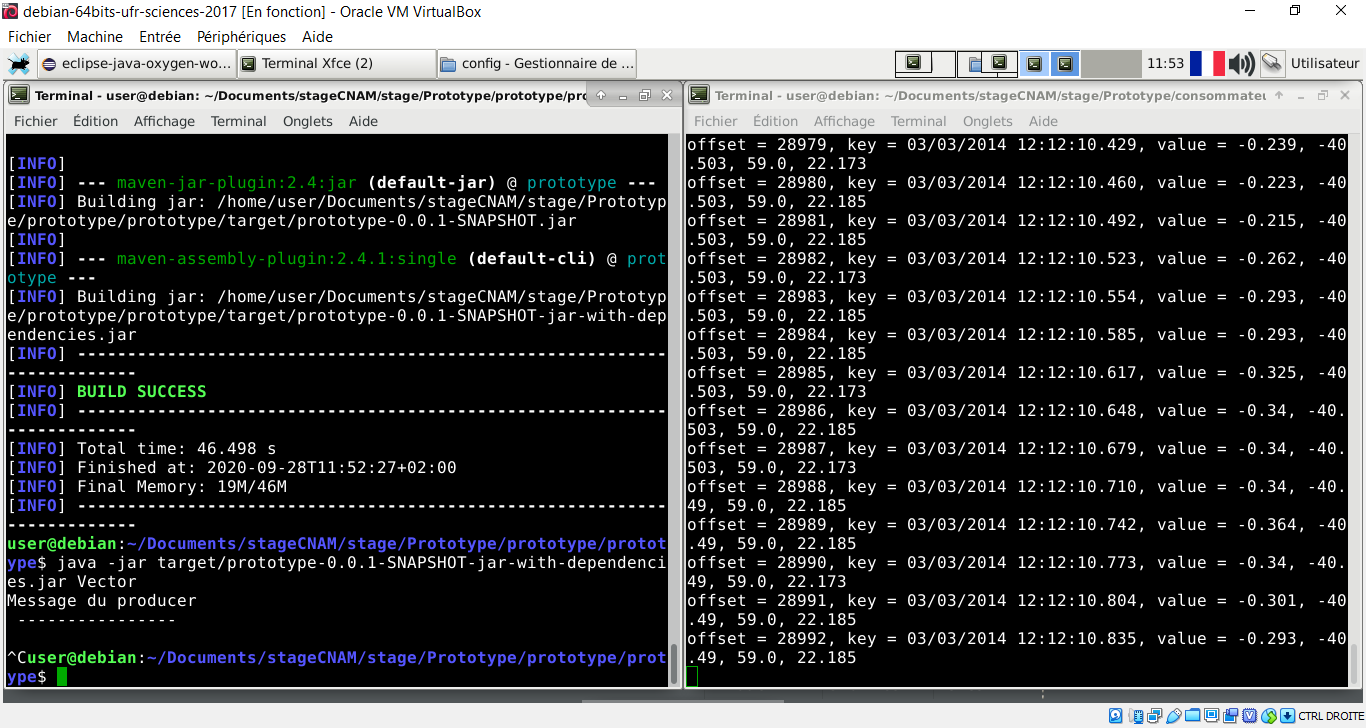
\includegraphics[scale=0.5]{../include/producteurConsommateur.PNG}
				\caption{Exemple d'exécution}
				\label{fig:exemple}
			\end{figure}
			Par exemple, la figure \ref{fig:exemple} montre une exécution du Producteur (à gauche) et du Consommateur (à droite) pour le topic "Vecteur".
			Ce topic permet d'obtenir la valeur des métriques "fréqence cardique, réponse électrodermale, température de la peau, rythme cardiaque" qui sont dans le champ \texttt{value}.
			Chaque log à pour clé le temps (date et heure d'acquisition).\par
			Tout le code pour ce prototype se trouve sur le Github \href{https://github.com/laurelinemartin/stage/Prototype}{https://github.com/laurelinemartin/stage/Prototype}.
	\subsection{Intégrer le prototype aux travaux déjà menés}\label{sec:travaux}
		Des travaux antérieurs ont été menés pour le projet global.
		Ces tavaux concernent en particulier la détection et la reconnaissance d'états émotionnels à partir de capteurs physiologiques.
		Cependant, les algorithmes utilisent des données préalablement acquises. 
		Autrement dit, les mesures physiologiques sont faites expérimentalement en laboratoire et elles sont enregistrées dans un fichier Excel (au format CSV) dans un premier temps.
		Et dans un second temps, les données sont analysées par les algorithmes qui ont été élaborés par des chercheurs du CEDRIC.
		En particulier Viviane GAL dans sa thèse \cite{gal_2019}.
		Il n'y a donc pas de notion de temps-réel dans ces travaux.
		C'est pour palier à ce problème que j'ai mis au point la solution que je présente ici.\par
		Nous présentons dans cette partie l'intégration de cette solution aux travaux qui ont déjà été menés.
		Pour cela, nous allons tout d'abord introduire les capteurs physiologiques qui sont utilisés par les travaux précédents.
		Cette introduction va nous permettre de trouver le connecteur adéquat pour ingérer les données des capteurs dans notre solution Kafka.
		Nous ferons la comparaison de différents connecteurs et nous nous positionnerons sur l'un d'entre.
		Puis, nous présenterons l'architecture de l'intégration de notre solution au projet.
		Enfin, nous ferons le bilan de ce qu'apporte notre prototype au projet.
		\subsubsection{Capteurs physiologiques utilisés}\label{sec:capteurs}
			Afin que notre prototype transmette les données provenant de capteurs aux algorithmes de reconnaissance des états émotionnels, nous devons nous adapter aux capteurs déjà utilisés par le laboratoire pour les expérimentations passées et futures.
			Nous n'avons pas la possibilité de changer les capteurs, alors c'est à notre solution de s'y adapter.\par
			Les capteurs physiologiques qui sont utilisés dans le projet sont des capteurs de chez TEA Ergo\footnote{\href{https://www.teaergo.com}{https://www.teaergo.com}}.
			Ce sont les capteurs Captiv présentés dans la Figure \ref{fig:capteurstea} des images issues du site\newline 
			\href{https://www.teaergo.com/fr/products/}{https://www.teaergo.com/fr/products/} que j'ai consulté le 28/09/20.
			\begin{figure}
				\begin{subfigure}{0.5\textwidth}
					\centering
					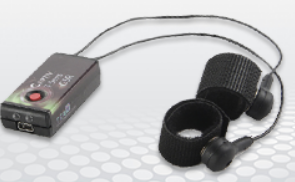
\includegraphics[scale=0.5]{../include/TEAgsr.PNG}
					\caption{Capteur pour la mesure de la réponse électrodermale}
					\label{fig:gsr}
				\end{subfigure}
				\begin{subfigure}{0.5\textwidth}
					\centering
					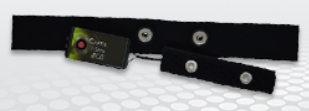
\includegraphics[scale=0.5]{../include/TEAhr.PNG}
					\caption{Capteur pour la mesure de la fréquence cardiaque}
					\label{fig:hr}
				\end{subfigure}\newline
				\begin{subfigure}{0.5\textwidth}
					\centering
					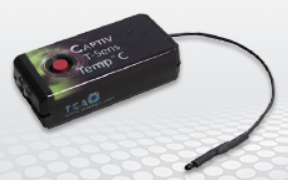
\includegraphics[scale=0.5]{../include/TEAbt.PNG}
					\caption{Capteur pour la mesure de la température à la surface de la peau}
					\label{fig:bt}
				\end{subfigure}
				\begin{subfigure}{0.5\textwidth}
					\centering
					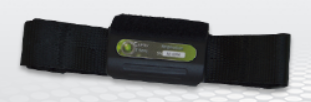
\includegraphics[scale=0.5]{../include/TEArr.PNG}
					\caption{Capteur pour la mesure de la fréquence respiratoire}
					\label{fig:rr}
				\end{subfigure}
				\caption{Les capteurs CAPTIV}
				\label{fig:capteurstea}
			\end{figure}
			Ceux que nous possédons permettent la mesure de la réponse électrodermale (Figure \ref{fig:gsr}), du rythme cardiaque (Figure \ref{fig:hr}), de la température à la surface de la peau (Figure \ref{fig:bt}) et de la fréquence respiratoir (Figure \ref{fig:rr}).
		\subsubsection{Connecteurs}\label{sec:connecteurs}
			Pour utiliser le prototype avec les travaux qui ont déjà été menés pour la recherche des états émotionnels, nous devons pouvoir utiliser des capteurs physiologiques comme sources de données.
			Pour cela, nous avons besoin d'utiliser un connecteur source.
			Ce connecteur permettra de faire le lien entre les capteurs physiologiques et le Producteur.
			Nous allons utiliser ConnectAPI proposé par Kafka pour faire ce "pont".
			Un connecteur nous permet de récupérer les données provenant des structures externes à Kafka pour les formaliser pour le Producteur.
			Ainsi, les données provenant de différentes sources pourront être utilisées dans Kafka.
			Utiliser un connecteur nous permet d'homogénéiser les données.
			En effet, les données proviennent de différentes sources, elles peuvnet donc être hétérogènes. 
			Les connecteurs permettent de formaliser ces données en un seul format compréhensible par le Producteur.
			De plus, utiliser un connecteur nous permet d'ajouter simplement un nouveau capteur (ou d'en supprimer un).
			Cela nous sera très utile pour de futurs travaux où nous ajouterons d'autres capteurs (capteurs dans l'environnement, par exemple des capteurs de présence).\par
			Une multitude de connecteurs existent déjà. 
			Il s'agit de connecteurs implémentés par Confluent (la plate-forme de Kafka) ou par la communauté.
			Sur le Confluent Hub\footnote{\href{https://www.confluent.io/hub/kafka-connectors-33}{https://www.confluent.io/hub/kafka-connectors-33}}, j'ai pu rechercher le connecteur qui convenait le mieux pour notre cas.
			Sur ce hub, 165 connecteurs sont répertoriés.
			Certains connecteurs permettent de récupérer des données sources provenant de structures extenes à Kafka, d'autres permettent d'évacuer les données vers des structures externes et d'autres permettent de transformer les données.
			Certains connecteurs permettent même de faire deux ou trois de ces types d'actions. 
			Dans le cadre de notre projet, je me suis intéressée ici aux connecteurs sources.
			Nous allons vous présenter les différents connecteurs sources que nous avons pu répertoriés.\par
			Pour notre recherche, nous avons appliqués les filtres suivants : \newline
			\texttt{Plugin type $=$ "Source" \& License $=$ "Free"}.\newline
			Comme indiqué plus haut, nous recherchons un connecteur source.
			De plus, nous avons préféré nous restreindre aux licences libres pour avoir au moins une vue sur le code qui est utilisé.\par
			La recherche nous a donné 38 connecteurs.
			Nous avons trié ces connecteurs en deux sous-parties :
			\begin{itemize}
				\item Les connecteurs potentiels : Les connecteurs qui peuvent servir pour notre cas, c'est-à-dire qui peuvnet faire de l’ingestion de données en temps-réel;
				\item Les connecteurs non-retenus : Les connecteurs jugés trop éloignés de notre cas d’usage pour des raisons diverses.
			\end{itemize}
			Les Tableaux \ref{tab:potentiels} et \ref{tab:connecteursnon} listent ces 38 connecteurs avec une petite description.\par
			\textbf{1. Les connecteurs potentiels}\par
			Ces connecteurs vont permettre de récupérer des données en temps-réel. 
			Comme nos capteurs diffusent en permanence, nous avons besoin d’un connecteur capable de transférer des données en temps-réel depuis les capteurs vers Kafka.
			\begin{table}[h]
				\begin{tabular}{|p{7.5cm}|p{7.5cm}|}
					\hline
					\rowcolor{lightgray} Connecteur & Description\\\hline
					Diffusion® Kafka Connector & Permettre aux clients web, mobile et IoT de consommer et envoyer des données temps-réel et orientées-événement\\\hline
					Kafka Connect Shell & Ingère la sortie d’une commande passé dans le shell vers Kafka (peut être utilisé avec un algorithme déjà implémentés de travaux antérieurs) \\\hline
				\end{tabular}
				\caption{Les connecteurs potentiels}
				\label{tab:potentiels}
			\end{table}
			Le tableau \ref{tab:potentiels} répertorie ces connecteurs.\par
			\textbf{2. Les connecteurs non-retenus}\par
			Ces connecteurs peuvent être écartés de nos recherches. 
			Ces plug-in sont soit trop spécifiques, soit orientés bases de données relationnelles, soit pour des fichiers systèmes, soit pour créer des données factices, etc.
			Le tableau \ref{tab:connecteursnon} répertorie ces connecteurs.
			\begin{longtable}{|p{7.5cm}|p{7.5cm}|}
				\hline
				\rowcolor{lightgray} Connecteur & Description\\\hline
				\endhead
				Kafka Connect JDBC & Pour les bases de données relationnelles JDBC\\\hline
				Kafka Connect JDBC with Flatten Feature & Extension de Kafka Connect JDBC\\\hline
				Debezium MySQL CDC Connector & Surveillance et enregistrement des changements pour MySQL server\\\hline
				Debezium PosgreSQL CDC Connector & Surveillance et enregistrement des changments pour les bases de données PostgreSQL\\\hline
				Debezium SQL server CDC Connector & Surveillance et enregistrement des changements pour des serveurs SQL\\\hline
				MongoDB Connector for Apache Kafka & Récupérer des données depuis une base de données MongoDB.\\\hline
				Debezium MongoDB CDC Connector & Surveillance des ensemble de réplicas MongoBD\\\hline
				Kafka Connect Spooldir & Pour des fichiers délimités de fichiers systèmes\\\hline
				Couchbase DB Connector & Transférer des données depuis et vers Couchbase server\\\hline
				Kafka Connect Crux & Transférer des données depuis et vers les nœuds Crux\\\hline
				Kafka Connect Venafi & Se connecter à Venafi Platform via HTTP et récupérer des événements logs depuis Kafka. Filtrage, transformation, traitement possible.\\\hline
				Kinetica DB Connector & Pour Kinetica, base de données distribuée en mémoire accélérée par GPU. Ingèrer, analyser et visualiser en même temps\\\hline
				SAP Hana Connector & Pour les systèmes SAP\\\hline
				Databricks Connector for Apache Kafka & Se connecter à une base de données Databricks et d'envoyer les données vers Kafka.\\\hline
				Levy Xenon Connector & Pour fort I/O et bigData\\\hline
				CockroachDB Change Data Capture & Fonctionnalité de capture de changement de ligne dans la BD\\\hline
				Hazelcast Jet Kafka Connector & Offre un producer et un consumer pour transférer des données entre Kafka et Hazelcast\\\hline
				StreamSets Data Collector & Simplifier la construction, l’éxecution et les opérations pour les flots de données\\\hline
				Kafka Connect IRC & Connecteur source pour IRC\\\hline
				Kafka Connect HTTP & Pour les APIs JSON/http\\\hline
				Kafka Connect Sound & Lire des données de microphone et envoyer des données pour sortie audio\\\hline
				Kafka Connect Reddit & Récupérer des posts et des commentaires en temps-réel via Reddit\\\hline
				Kafka Connect FileSystem & Lire différents formats de fichiers de différents types de fichiers système\\\hline
				Kafka Connect Common Transfomations & Transformation de données de fichiers.\\\hline
				Kafka connect-pulsar & Permet de répliquer des données de Apache Pulsar vers Apache Kafka\\\hline
				Kafka Connect Maxmind Transformation & Pour ajouter des données GeoIP aux données Kafka\\\hline
				Kafka Connect Twitter & Flux de données Twiitter vers Kafka\\\hline
				Kafka Connect Email & POM parent pour les projets Kafka Connect\\\hline
				Kafka Connect Simulator & Générer des données de test\\\hline
				Kafka Connect RSS Source & Récupérer des données de flux RSS et Atom\\\hline
				Kafka Connect Flume Avro & Envoyer des données depuis Apache Flume\\\hline
				Voluble & Générateur de données factices\\\hline
				Apache Connect IoT Hub & Pour Azur IoT Hub\\\hline
				Kafka Connect Zeebe	& Enregistrements de workflow BPMN vers kafka\\\hline
				Kafka Connect File Pulse & Parse, transfomer et charger les données  depuis un fichier système local vers Kafka\\\hline
				\caption{Les connecteurs non-retenus}
				\label{tab:connecteursnon}
			\end{longtable}\par
			\textbf{3. Positionnement}\par
			Parmi les deux connecteurs que j'ai retenus, nous avons décidé d'utiliser le connecteur \texttt{Kafka Connect Shell}\footnote{\href{https://www.confluent.io/hub/thomaskwscott/kafka-connect-shell-source}{https://www.confluent.io/hub/thomaskwscott/kafka-connect-shell-source}}.
			Dans l'optique d'être plus rapide dans nos tests, ce connecteur nous semble être le meilleur choix.
			Nous allons l'utiliser avec un algorithme déjà existant provenant de travaux antérieurs pour le projet qui affiche les données des capteurs dans un terminal.
			Avec le connecteur Kafka Connect Shell, nous serons capables de lire les données affichées sur le terminal et de les transmettre au Producteur Kafka.
		\subsubsection{Schéma de l'intégration du prototypes aux travaux déjà menés}\label{sec:schematravaux}
			\begin{figure}
				\centering
				\vspace*{-1cm}
				\rotatebox{90}{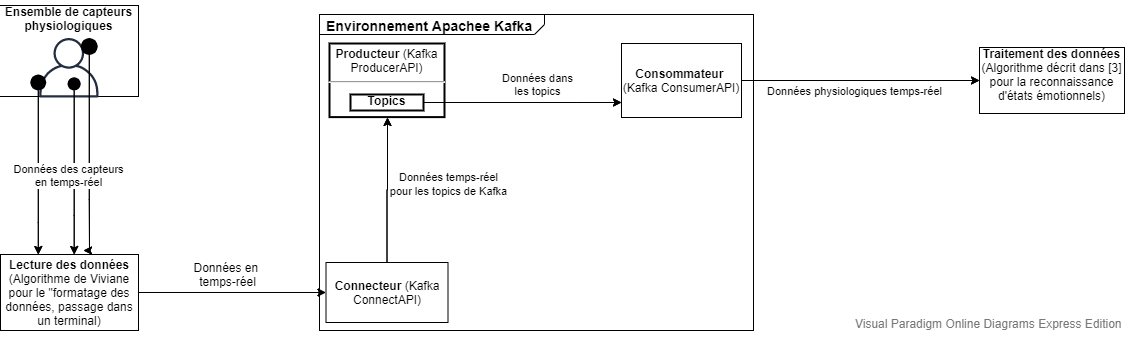
\includegraphics[scale=0.75]{../include/schema-global.jpg}}
				\caption{Schéma de l'architecture du prototype intégré au projet}
				\label{fig:archiglobale}
			\end{figure}
			L'architecture présentée à la Figure \ref{fig:archiglobale} nous permet de voir l'intégration de notre solution aux travaux menés précédemment.
			Comme il existe déjà un algorithme qui permet de lire les données des capteurs et de les afficher sur un terminal, nous l'utilisons.
			Le Connecteur que nous utilisons permet de récupérer des données sur un terminal et de les transmettre au Producteur sous la bonne forme pour être envoyées dans les topics.
			Les topics sont ensuite consommés par les algorithmes de reconnaissance de l'état émotionnel.
	\subsection{Validation}\label{sec:validation}
		L'objectif que nous avions pour ce prototype était de pouvoir récupérer des données provenant de capteurs et de les envoyer vers les algorithmes de détection et de reconnaissance d'états émotionnels.\par
		Dans ce rapport, je propose une solutiion que j'ai implémentée.
		Cette solution est actuellement testée avec un fichier au format CSV contenant les données de quatre capteurs physiologiques : la fréquence respiratoire, la réponse électrodermale, la température corporelle et la fréquence cardiaque. 
		Chaque ligne de ce fichier est envoyée dans les topics avec 30ms d'écart.
		Ces 30 ms correspondent au temps moyen d'acquisition entre deux données.
		Cela nous donne une impression de temps-réel. 
		Les données sont ensuite lues par un consommateur qui les affiche au fur et à mesure dans un terminal.\par
		Nous avons présenter un connecteur permettant d'éliminer à terme le fichier de données acquisent préalablement dans le but de travailler directement avec des données de capteurs physiologiques.
		Nous avons aussi présentés comment le prototype pouvait être intégrés aux travaux déjà réalisés au laboratoire CEDRIC.\par
		L'objectif de ce prototype est d'ingérer et de distribuer les données temps-réel provenant de capteurs.
		Du point de vue de cet objectif, nous pouvons dire que cette implémentation correspond à ce que nous voulions réaliser.
		Les données sont lues et puis renvoyées dans différents topics pour être analyses.
		Pouvoir séparer les données de différentes métriques nous permet de les analysées séparément ou ensemble selon les besoins.
		De plus, cela nous permettra dans de futurs travaux de séparer les données physiologiques d'autres données de capteurs pour le jeu.\par

\section{Conclusion}\label{sec:conclusion}
	L'objectif principal de ce projet est de réaliser un jeu pervasif adaptable dynamiquement aux joueur en tenant compte de leurs états émotionnels.
	Pour la détection et la reconnaissance d'états émotionnels, nous souhaitons utiliser des capteurs physiologiques.
	Ces capteurs génèrent des données qui sont analysées par des algorithmes pour détecter et reconnaître les états émotionnels des joueurs au cours du jeu.
	Une fois l'état émotionnel reconnu, le jeu peut alors proposer au joueur l'événement le plus adapté pour garantir le meilleur divertissement possible aux joueurs.
	Avec cet objectif en tête, nous avons cherché une solution efficace de gérer les données fournies en continu par les capteurs.\par
	Dans ce rapport, nous avons présenté plusieurs travaux qui ont été menés tout au long de ce stage.
	Cette contribution a été, avant tout, l'occasion d'affiner les besoins pour la conception d'un jeu pervasif adaptable aux états émotionnels du joueur.
	En premier lieu, nous avons conçu un cadre de comparaison pour l'adaptation dynamique de jeux à leurs utilisateurs que nous présentons dans notre état de l'art.
	Puis, nous avons abordé la notion d'expérience utilisateur dans le domaine du jeu et l'expérimentation que nous avons mené lors d'un escape game.
	Ensuite, nous avons présenté notre première tentative de contribution sous la forme d'un modèle conceptuel pour représenter l'adaptation d'un jeu pervasif aux états émotionnels d'un joueur.
	Enfin, nous avons présenté le prototype de notre solution pour la gestion des données provenant de capteurs physiologiques pour que ces données soient utilisées avec des algorithmes déjà existants.
	Cette dernière contribution que nous avons détaillée dans ce rapport a été implémentée.
	Elle permet de lire et d'envoyer en temps-réel (avec le minimum de latence possible) les données sur des topics.\par
	% Plus d'une fois j'ai eu envie de me jeter par la fenêtre. Clairement les pire 8 mois de toute ma vie. Et pourtant j'en ai vu des choses. Je veux crever très clairement. A chaque fois que je regarde ce rapport, j'ai envie de pleurer. Je fais un vrai blocage sur ce travail. Juste laissez moi tranquille en fait. Je ne sais même pas ce qu'on me demande là, juste j'applique bêtement.
	Ce travail a été l'occasion d'affiner les contours du projet.
	Plusieurs perspectives sont a envisager.
	Tout d'abord il faudrait mettre à l'épreuve notre prototype directement avec nos capteurs.
	Si les tests avec les capteurs sont satisfaisants, alors il sera possible d'utiliser des algorithmes pour la détection et la reconnaissance d'états émotionnels en temps-réel.
	Il sera aussi envisageable de passer à l'étape de la conception d'algorithmes pour l'adaptation dynamique du jeu selon l'état émotionnel courant du joueur.
	Il faudra par la suite développer d'autres aspects liés au jeu lui-même.
	Comme par exemple la jouabilité ou le game design.
	Un objectif de ce projet est d'utiliser ce jeu pour d'autres domaines d'applications que celui du divertissement.
	On peut imaginer utiliser ce jeu pour enseigner des émotions par exemple.
	Il faudra donc garder un aspect très générique de ce jeu.


\newpage
\bibliographystyle{abbrv}
\bibliography{../include/biblio}
\medskip

\hspace*{-1cm}
\Large{\textbf{Sitographie :}}\newline
\href{https://www.usabilis.com/definition-ux-experience-utilisateur-user-experience/}{https://www.usabilis.com/definition-ux-experience-utilisateur-user-experience/}\newline
\href{https://www.upsolver.com/blog/kafka-versus-rabbitmq-architecture-performance-use-
case}{https://www.upsolver.com/blog/kafka-versus-rabbitmq-architecture-performance-use-
case} \textit{[en]} \medskip\newline
\href{https://blog.ippon.fr/2018/03/27/comparatif-rabbitmq-kafka/}{https://blog.ippon.fr/2018/03/27/comparatif-rabbitmq-kafka/} \textit{[fr]}\medskip\newline
\href{https://www.cloudamqp.com/blog/2015-05-18-part1-rabbitmq-for-beginners-what-is-rabbitmq.htm}{https://www.cloudamqp.com/blog/2015-05-18-part1-rabbitmq-for-beginners-what-is-rabbitmq.htm} \textit{[en]}\medskip\newline
\href{https://openclassrooms.com/fr/courses/4451251-gerez-des-flux-de-donnees-temps-reel/4451521-metamorphosez-vos-applications-temps-reel-avec-kafka}{https://openclassrooms.com/fr/courses/4451251-gerez-des-flux-de-donnees-temps-reel/4451521-metamorphosez-vos-applications-temps-reel-avec-kafka} \textit{[en]}\newline

\hspace*{-1cm}
\Large{\textbf{Videographie :}}\newline
	"L'expérience utilisateur dans la création de jeux vidéo (C. Hodent)"\newline
	"Démarches et méthodes pour la conception de l'expérience utilisateur - LuxI/O 2018"\newline
	"How Games Move Us: Emotion by Design | Katherin Isbister | TEDxHarkerSchool"\newline
	"Of Brains and Interfaces - Celia Hodent - Netexplo  Forum 2018 - UNESCO"
	Sur \href{http://youtube.fr}{htpp://youtube.fr}\par

\newpage
\appendix
\renewcommand{\appendixpagename}{Annexes}\appendixpage
% \section{Adaptation d’un jeu pervasif particularisé basée sur l'état émotionnel et sur les caractéristiques du joueur – État de l’art}\label{ann:eda}
%	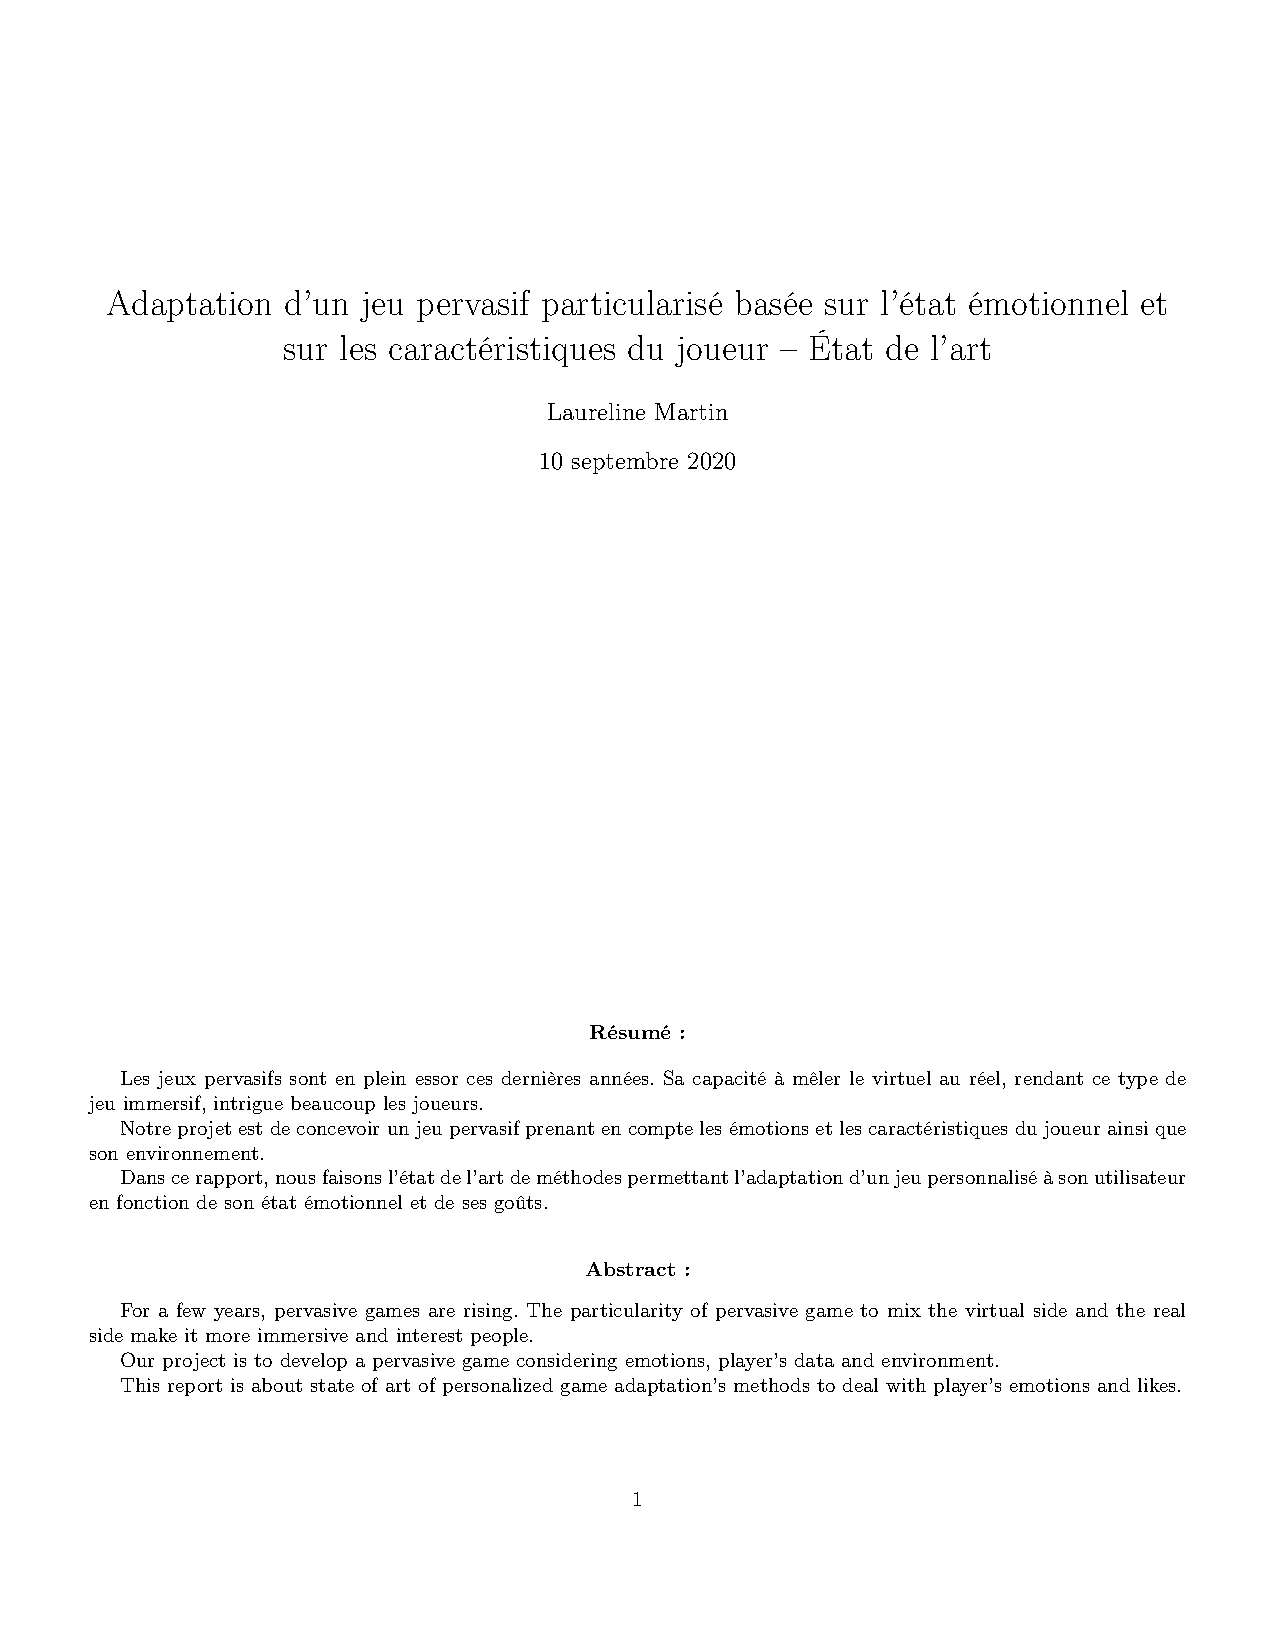
\includepdf[pages=-]{../include/eda.pdf}

\section{Description des capteurs}
	

\section{Présentation du laboratoire CEDRIC}\label{ann:cedric}
	Avant de présenter le travail réalisé, nous allons faire une présentation du laboratoire CEDRIC.
	Le laboratoire de Centre d'Etudes et De Recherche en Informatique et Communication (CEDRIC)\footnote{\href{http://cedric.cnam.fr/lab/accueil/labo/}{http://cedric.cnam.fr/lab/accueil/labo/}} au sein du Conservatoire National des Arts et Métiers (CNAM) de Paris\footnote{\href{http://www.cnam.fr/portail/accueil-conservatoire-national-des-arts-et-metiers-821166.kjsp}{http://www.cnam.fr/portail/accueil-conservatoire-national-des-arts-et-metiers-821166.kjsp}} se situe au 2 rue Conte 75003 PARIS.\par
	Le laboratoire CEDRIC est composé de huit équipes menant des recherches et des actions dans le domaine de l'informatique fondamentale et appliquée, ainsi que dans d'autres disciplines proches telles que les statistiques, électronique,....\par
	Les équipes du laboratoire sont les suivantes :
	\begin{itemize}
		\item L'équipe Données complexes, apprentissage et représentations (Vertigo) : Extraire de l'information et construire des méthodes de gestion de données basées sur le contenu pour des données massives audios, images et vidéos;
		\item L'équipe Interactivité pour Lire et Jouer (ILJ) : Questions autour de l'interaction Homme-Machine concernant des activités telles que le jeu et la lecteure. Cette équipe mèle plusieurs disciplines (l'informatiques, la psychologie, le design, les arts,...) afin de répondre aux études en cours qui concernent la modélisation de la difficulté dans les jeux, les méthodologies de game design inclusif, etc.;
		\item L'équipe Ingénieries des Systèmes d'Information et de Décision (ISID) : Cette équipe s'est réunie autour de trois axes de recherche : les systèmes décisionnels, le web sémantique et la qualité des systèmes d'information. Son but est de concevoir des méthodes, des outils et des techniques	pour la conception et l'analyse de systèmes d'information et de décision dans tous les domaines;
		\item L'équipe Traitement du signal et architectures électroniques (LAETITIA) : Concentrée sur trois axes de recherhe : le traitement du signal pour les télécommunications (recherches en lien avec les réseaux cellulaires (5G/6G) et en lien avec les problématiques de couches physique pour les réseaux faible puissance longue portée pour l'IoT), la sûreté de fonctionnement des sytèmes dynémiques (recherche en automatique) et l'implémentation temps-réel (mise en oeuvre des algorithmes proposés par l'équipe);
		\item L'équipe Méthode Statistique de Data-Mining et Apprentissage (MSDMA) : Traitement de données et développement de modèles d'apprentissage statistiques dans le but d'extraire des informations pour prise de décision;
		\item L'équipe Optimisation Combinatoire (OC) : Rassemblée autour de deux axes : la programmation mathématique et applications ainsi que les graphes et optimisation;
		\item L'équipe Réseaux et Objets Connectés (ROC) : Porte sur l'analyse et l'exploitation des nouvelles architectures réseaux et des systèmes liés à la virtualisation, à la mobilité et au développement des objets connectés;
		\item L'équipe Systèmes Sûrs (SYS) : Spécialisation, conception, vérification et évaluation des systèmes. Pour cela, Les recherches se font autour de trois axes : l'axe typage, sémantique et preuve, l'axe architecture logiciel, architecture systèmes et ligne de produit et l'axe vérification et évaluation de systèmes parallèles et asynchrones.
	\end{itemize}

\newpage
\section{Ressources pour définir la notion d'expérience utilisateur}\label{ann:ux}
	\textbf{Sitographie :}\newline
	% \href{https://fr.wikipedia.org/wiki/experience_utilisateur#definitions}{https://fr.wikipedia.org/wiki/experience_utilisateur#Definitions}\newline
	\href{https://www.usabilis.com/definition-ux-experience-utilisateur-user-experience/}{https://www.usabilis.com/definition-ux-experience-utilisateur-user-experience/}\par
	\textbf{Videographie :}\newline
	"L'expérience utilisateur dans la création de jeux vidéo (C. Hodent)"\newline
	"Démarches et méthodes pour la conception de l'expérience utilisateur - LuxI/O 2018"\newline
	"How Games Move Us: Emotion by Design | Katherin Isbister | TEDxHarkerSchool"\newline
	"Of Brains and Interfaces - Celia Hodent - Netexplo  Forum 2018 - UNESCO"
	Sur \href{http://youtube.fr}{htpp://youtube.fr}\par
	\textbf{Bibliographie :}\newline
	Olga Vl. Bitkina, Hyun K. Kim, Jaehyun Park \textit{Usability and user experience of medical devices: An overview of thecurrent state, analysis methodologies, and future challenges} International Journal of Industrial Ergonomics 76, 2020.

% \newpage
% \section{Description détaillée des classes de l'ontologie}\label{ann:detailclasses}
%	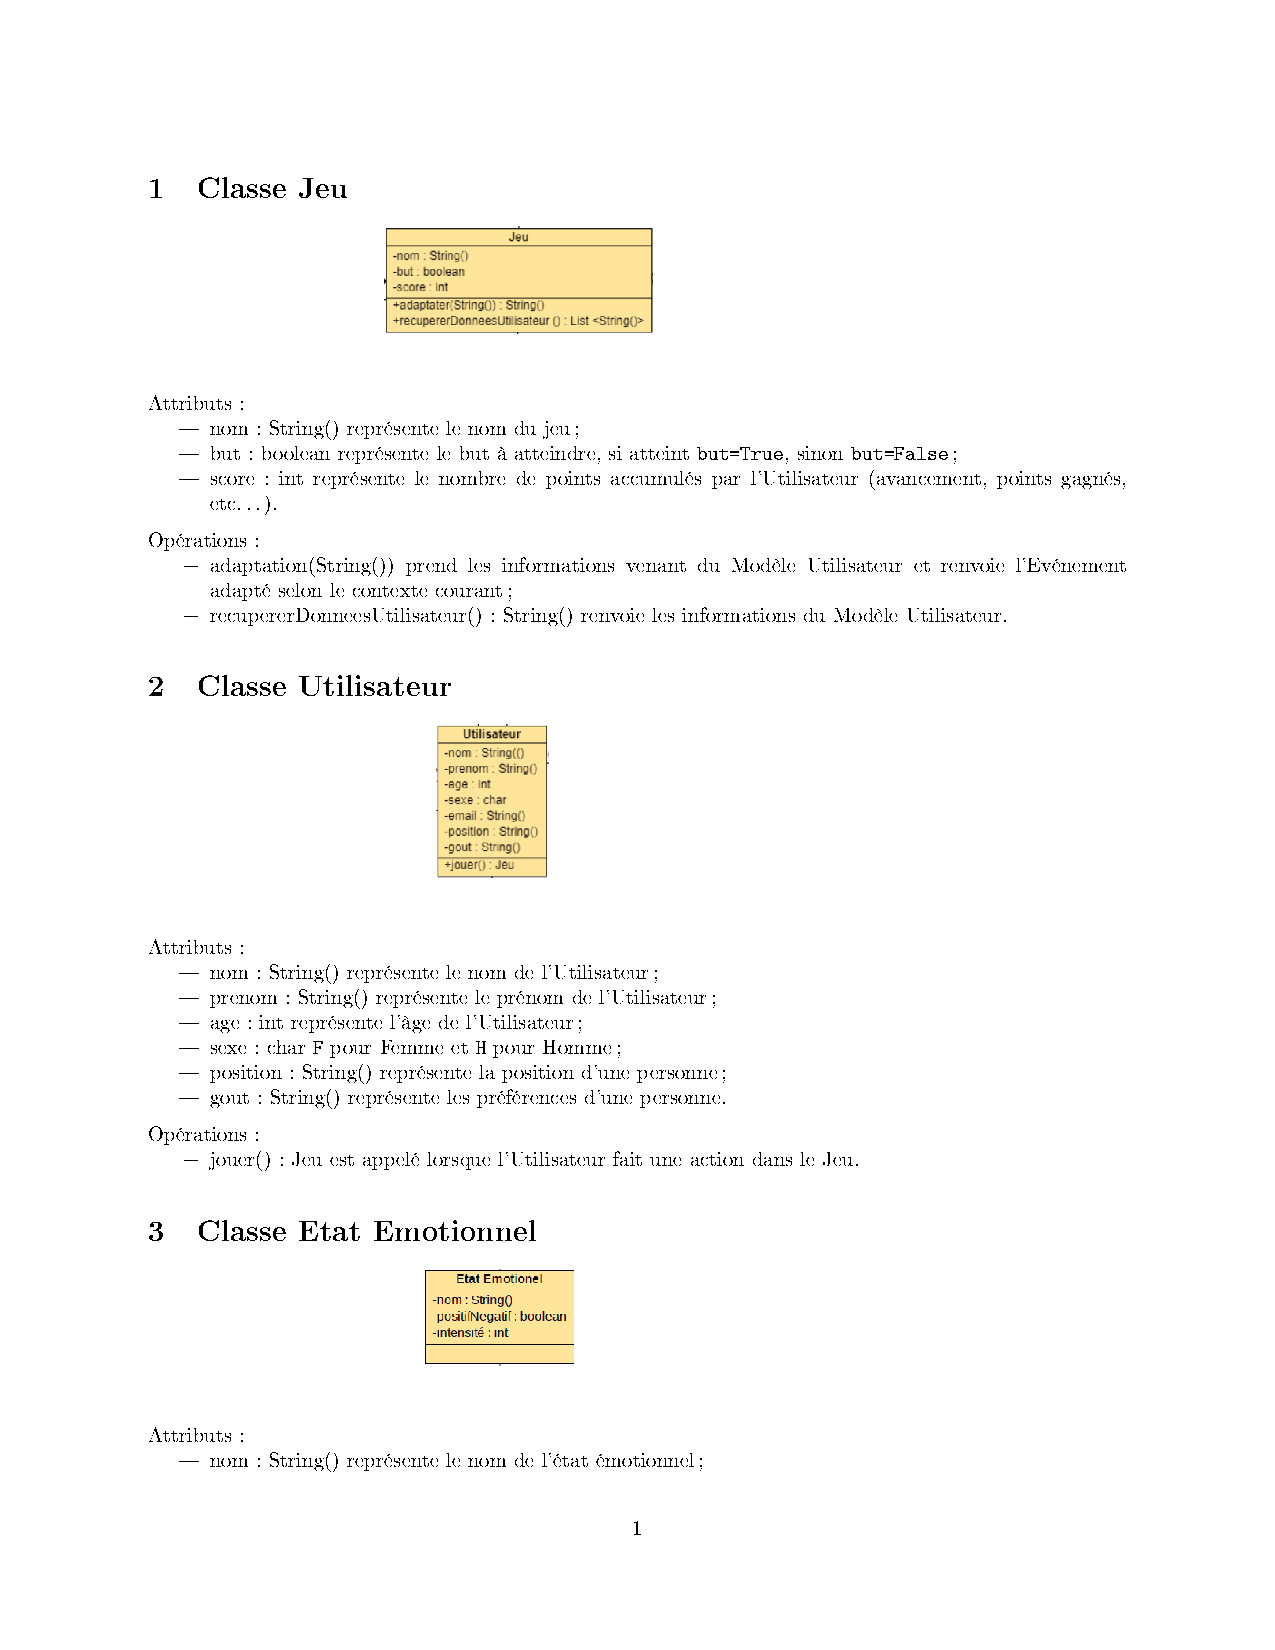
\includepdf[pages=-]{../include/descriptionClassesOntologie.pdf}

\newpage
\section{Sitographie pour la construction de la synthèse comparative entre Kafka et RabbitMQ}\label{ann:kafkarabbitmq}
	\hspace*{-0.5cm}\href{https://www.upsolver.com/blog/kafka-versus-rabbitmq-architecture-performance-use-
	case}{https://www.upsolver.com/blog/kafka-versus-rabbitmq-architecture-performance-use-
	case} \textit{[en]} \medskip\newline
	\href{https://blog.ippon.fr/2018/03/27/comparatif-rabbitmq-kafka/}{https://blog.ippon.fr/2018/03/27/comparatif-rabbitmq-kafka/} \textit{[fr]}\medskip\newline
	\href{https://www.cloudamqp.com/blog/2015-05-18-part1-rabbitmq-for-beginners-what-is-rabbitmq.htm}{https://www.cloudamqp.com/blog/2015-05-18-part1-rabbitmq-for-beginners-what-is-rabbitmq.htm} \textit{[en]}\medskip\newline
	\href{https://openclassrooms.com/fr/courses/4451251-gerez-des-flux-de-donnees-temps-reel/4451521-metamorphosez-vos-applications-temps-reel-avec-kafka}{https://openclassrooms.com/fr/courses/4451251-gerez-des-flux-de-donnees-temps-reel/4451521-metamorphosez-vos-applications-temps-reel-avec-kafka} \textit{[en]}

\newpage
\section{Offre de stage}\label{app:annexe1}
	\textbf{Elaboration du modèle conceptuel des jeux pervasifs adaptables avec la prise en compte des états émotionnels des joueurs}\par
	\medskip
	\textbf{Contexte :}\newline
	Le champ des jeux affectifs est nouveau. Il s’appuie sur l’intégration de nouveaux moyens à développer dans les jeux afin d’adaptabilité. [1] et [2] présentent une méthodologie unifiée pour la conception des jeux affectifs utilisant le plus tôt possible le mécanisme de boucle émotionnelle. Ils repèrent des variations à l’aide de mesures physiologiques et appliquent un modèle issu d’un ensemble construit considéré comme en relation avec les émotions. Leur étude montre combien la dimension émotionnelle de l’utilisateur est importante mais difficile à gérer.\newline
	Le profil du joueur, y compris ses émotions, impacte la conception des jeux. Afin de proposer une meilleure expérience aux joueurs et de proposer un jeu particularisé, le jeu doit être adaptable en fonction du contexte global du joueur. Nous sommes dans une approche holistique qui combine à la fois l’individu et ses émotions, et, les influences de l’entourage qui va du bâtiment lui-même à l’atmosphère que dégage le lieu. Très peu de travaux ont été faits pour la conception et le développement des jeux adaptables dynamiquement. [3] formalise le concept des jeux appliqués aux visites de musées. Ce travail modélise le jeu de visite et propose un processus d’équilibrage entre la dimension ludique et la dimension non ludique (la visite) de ce type de jeux. [3] propose des patrons de mission qui servent d’éléments réutilisables lors de la conception des jeux, mais qui ne couvrent qu’une partie du processus de conception.\par
	\textbf{Sujet :}\newline
	Il s’agit dans ce stage d’élaborer un modèle conceptuel du jeu pervasif adaptable basé sur les émotions. Ce modèle, éventuellement réalisé sous forme d’une ontologie, doit couvrir toute la variété des facteurs qui impactent le jeu tels que le profil de l’utilisateur et ses données physiologiques exprimant son état émotionnel. Cette ontologie doit être construite de façon à ce qu’elle soit adaptée à la démarche situationnelle nécessaire pour la composition dynamique du jeu.

\end{document}